% =====================================================================
%  JOURNAL SWITCHBOARD - change only this block when re-targeting the paper
% =====================================================================
\documentclass[12pt,a4paper]{article}          % JQAS: 11-12 pt, single column, double spaced
\usepackage[margin=1in]{geometry}
\usepackage{setspace}\doublespacing            % JQAS / Sage require double spacing; use \onehalfspacing or \singlespacing otherwise
\usepackage[authoryear,round]{natbib}          % Harvard (author-year). For numeric journals: \usepackage[numbers,sort&compress]{natbib}
\bibliographystyle{apalike}                     % Harvard-like. Numeric alternative: plainnat / vancouver / unsrtnat
\newcommand{\journalname}{Journal of Quantitative Analysis in Sports}
\newcommand{\anonymous}{false}                  % set to true for double-anonymised review copies
% =====================================================================
\usepackage[T1]{fontenc}\usepackage[utf8]{inputenc}
\usepackage{amsmath,amssymb,bm}
\usepackage{graphicx,booktabs,multirow,array,tabularx,longtable}
\usepackage{caption,subcaption,float}
\usepackage[hidelinks]{hyperref}\usepackage{url}
\usepackage{xcolor}\usepackage{siunitx}
\graphicspath{{figures/}}
\newcommand{\nRawRows}{25,396}
\newcommand{\nPlayerSeasons}{20,547}
\newcommand{\nAllPlayers}{3,817}
\newcommand{\nDebutWindow}{2,381}
\newcommand{\nGamesFortytwo}{1,833}
\newcommand{\nPlayers}{1,676}
\newcommand{\nObs}{13,193}
\newcommand{\nActive}{17}
\newcommand{\minActiveSeason}{15}
\newcommand{\sdPerLowMp}{14.9}
\newcommand{\sdPerHighMp}{4.1}
\newcommand{\minSpan}{2}
\newcommand{\maxSpan}{23}
\newcommand{\nGapPlayers}{458}
\newcommand{\pctGapPlayers}{27.3}
\newcommand{\nGapSeasons}{798}
\newcommand{\nSpanSeasons}{13,991}
\newcommand{\pctGapSeasons}{5.7}
\newcommand{\muPer}{13.67}
\newcommand{\sdPer}{4.32}
\newcommand{\skewPer}{0.39}
\newcommand{\nDev}{1,341}
\newcommand{\nHeld}{335}
\newcommand{\nDrafted}{1,336}
\newcommand{\medianSeasons}{7}
\newcommand{\meanSeasons}{7.9}
\newcommand{\nGrid}{720}
\newcommand{\pcaVar}{96}
\newcommand{\rmseHeld}{0.74}
\newcommand{\rmseHeldSd}{0.06}
\newcommand{\rmseTrain}{0.43}
\newcommand{\rmseLinear}{2.24}
\newcommand{\rmsePlayerMean}{2.76}
\newcommand{\rmseGlobal}{4.35}
\newcommand{\rmseHeldEight}{1.23}
\newcommand{\rmseHeldSixteen}{0.95}
\newcommand{\rmseHeldThirtytwo}{0.80}
\newcommand{\rmseHeldOneTwoEight}{0.74}
\newcommand{\bestEpoch}{361}
\newcommand{\nParams}{179,073}
\newcommand{\rmseOld}{2.23}
\newcommand{\selDbcvKdev}{7}
\newcommand{\selDbcvKho}{7}
\newcommand{\selDbcvKall}{13}
\newcommand{\selDbcvNoiseho}{1}
\newcommand{\selSilKdev}{24}
\newcommand{\selSilKho}{23}
\newcommand{\selSilKall}{14}
\newcommand{\selSilNoiseho}{56}
\newcommand{\selCompKdev}{14}
\newcommand{\selCompKho}{14}
\newcommand{\selCompKall}{7}
\newcommand{\selCompNoiseho}{29}
\newcommand{\gridKmin}{2}
\newcommand{\gridKmax}{33}
\newcommand{\ariSingleMin}{0.32}
\newcommand{\ariSingleMax}{0.66}
\newcommand{\ariAeSeedsMin}{0.09}
\newcommand{\ariAeSeedsMax}{0.38}
\newcommand{\kSingleMin}{2}
\newcommand{\kSingleMax}{27}
\newcommand{\bigShareEomMax}{63}
\newcommand{\bigShareEomMin}{33}
\newcommand{\noiseLeafMean}{34}
\newcommand{\noiseEomMean}{14}
\newcommand{\configList}{C1: 10,10,0.0,25,15; C2: 5,15,0.0,30,10; C3: 5,20,0.0,22,7; C4: 2,15,0.0,40,5}
\newcommand{\aeAllK}{3}
\newcommand{\aeAllSil}{0.48}
\newcommand{\aeAllPac}{0.57}
\newcommand{\aeAllStable}{80}
\newcommand{\aeAllSilEight}{0.44}
\newcommand{\aeAllPacEight}{0.32}
\newcommand{\aeAllStableEight}{67}
\newcommand{\aeAllRsqEight}{0.50}
\newcommand{\aeAllRsq}{0.37}
\newcommand{\aeSeedZeroK}{3}
\newcommand{\aeSeedZeroSil}{0.90}
\newcommand{\aeSeedZeroPac}{0.17}
\newcommand{\aeSeedZeroStable}{100}
\newcommand{\aeSeedZeroSilEight}{0.78}
\newcommand{\aeSeedZeroPacEight}{0.13}
\newcommand{\aeSeedZeroStableEight}{95}
\newcommand{\aeSeedZeroRsqEight}{0.50}
\newcommand{\aeSeedZeroRsq}{0.41}
\newcommand{\aeNostdK}{3}
\newcommand{\aeNostdSil}{0.56}
\newcommand{\aeNostdPac}{0.50}
\newcommand{\aeNostdStable}{94}
\newcommand{\aeNostdSilEight}{0.45}
\newcommand{\aeNostdPacEight}{0.31}
\newcommand{\aeNostdStableEight}{70}
\newcommand{\aeNostdRsqEight}{0.57}
\newcommand{\aeNostdRsq}{0.46}
\newcommand{\aeUmapK}{3}
\newcommand{\aeUmapSil}{0.71}
\newcommand{\aeUmapPac}{0.38}
\newcommand{\aeUmapStable}{95}
\newcommand{\aeUmapSilEight}{0.38}
\newcommand{\aeUmapPacEight}{0.33}
\newcommand{\aeUmapStableEight}{49}
\newcommand{\aeUmapRsqEight}{0.29}
\newcommand{\aeUmapRsq}{0.24}
\newcommand{\aeHdbK}{5}
\newcommand{\aeHdbSil}{0.43}
\newcommand{\aeHdbPac}{0.76}
\newcommand{\aeHdbStable}{66}
\newcommand{\aeHdbSilEight}{0.36}
\newcommand{\aeHdbPacEight}{0.76}
\newcommand{\aeHdbStableEight}{66}
\newcommand{\aeHdbRsqEight}{0.18}
\newcommand{\aeHdbRsq}{0.18}
\newcommand{\summK}{4}
\newcommand{\summSil}{0.93}
\newcommand{\summPac}{0.08}
\newcommand{\summStable}{99}
\newcommand{\summSilEight}{0.90}
\newcommand{\summPacEight}{0.07}
\newcommand{\summStableEight}{99}
\newcommand{\summRsqEight}{0.60}
\newcommand{\summRsq}{0.47}
\newcommand{\summWardK}{3}
\newcommand{\summWardSil}{0.49}
\newcommand{\summWardPac}{0.62}
\newcommand{\summWardStable}{96}
\newcommand{\summWardSilEight}{0.47}
\newcommand{\summWardPacEight}{0.33}
\newcommand{\summWardStableEight}{81}
\newcommand{\summWardRsqEight}{0.55}
\newcommand{\summWardRsq}{0.42}
\newcommand{\rawK}{3}
\newcommand{\rawSil}{0.93}
\newcommand{\rawPac}{0.10}
\newcommand{\rawStable}{99}
\newcommand{\rawSilEight}{0.85}
\newcommand{\rawPacEight}{0.10}
\newcommand{\rawStableEight}{97}
\newcommand{\rawRsqEight}{0.72}
\newcommand{\rawRsq}{0.57}
\newcommand{\pcaK}{3}
\newcommand{\pcaSil}{0.74}
\newcommand{\pcaPac}{0.31}
\newcommand{\pcaStable}{94}
\newcommand{\pcaSilEight}{0.50}
\newcommand{\pcaPacEight}{0.24}
\newcommand{\pcaStableEight}{80}
\newcommand{\pcaRsqEight}{0.34}
\newcommand{\pcaRsq}{0.14}
\newcommand{\dtwK}{3}
\newcommand{\dtwSil}{0.76}
\newcommand{\dtwPac}{0.34}
\newcommand{\dtwStable}{97}
\newcommand{\dtwSilEight}{0.36}
\newcommand{\dtwPacEight}{0.35}
\newcommand{\dtwStableEight}{70}
\newcommand{\dtwRsqEight}{0.66}
\newcommand{\dtwRsq}{0.53}
\newcommand{\aeEightK}{3}
\newcommand{\aeEightSil}{0.50}
\newcommand{\aeEightPac}{0.55}
\newcommand{\aeEightStable}{90}
\newcommand{\aeEightSilEight}{0.34}
\newcommand{\aeEightPacEight}{0.35}
\newcommand{\aeEightStableEight}{46}
\newcommand{\aeEightRsqEight}{0.48}
\newcommand{\aeEightRsq}{0.40}
\newcommand{\aeSixteenK}{4}
\newcommand{\aeSixteenSil}{0.57}
\newcommand{\aeSixteenPac}{0.41}
\newcommand{\aeSixteenStable}{86}
\newcommand{\aeSixteenSilEight}{0.35}
\newcommand{\aeSixteenPacEight}{0.32}
\newcommand{\aeSixteenStableEight}{53}
\newcommand{\aeSixteenRsqEight}{0.48}
\newcommand{\aeSixteenRsq}{0.38}
\newcommand{\aeThirtytwoK}{3}
\newcommand{\aeThirtytwoSil}{0.62}
\newcommand{\aeThirtytwoPac}{0.46}
\newcommand{\aeThirtytwoStable}{91}
\newcommand{\aeThirtytwoSilEight}{0.37}
\newcommand{\aeThirtytwoPacEight}{0.33}
\newcommand{\aeThirtytwoStableEight}{50}
\newcommand{\aeThirtytwoRsqEight}{0.49}
\newcommand{\aeThirtytwoRsq}{0.39}
\newcommand{\aeOneTwoEightK}{3}
\newcommand{\aeOneTwoEightSil}{0.70}
\newcommand{\aeOneTwoEightPac}{0.39}
\newcommand{\aeOneTwoEightStable}{92}
\newcommand{\aeOneTwoEightSilEight}{0.49}
\newcommand{\aeOneTwoEightPacEight}{0.29}
\newcommand{\aeOneTwoEightStableEight}{71}
\newcommand{\aeOneTwoEightRsqEight}{0.46}
\newcommand{\aeOneTwoEightRsq}{0.39}
\newcommand{\summSilTwo}{0.98}
\newcommand{\summSilFour}{0.93}
\newcommand{\summSilTwelve}{0.59}
\newcommand{\aeAllSilThree}{0.48}
\newcommand{\aeAllSilTwelve}{0.34}
\newcommand{\aeAllPacThree}{0.57}
\newcommand{\nMembersAe}{40}
\newcommand{\nMembersSumm}{8}
\newcommand{\mainK}{4}
\newcommand{\fourNA}{369}
\newcommand{\fourPerA}{16.5}
\newcommand{\fourSeasA}{12}
\newcommand{\fourASA}{52}
\newcommand{\fourStabA}{0.98}
\newcommand{\fourNB}{560}
\newcommand{\fourPerB}{12.5}
\newcommand{\fourSeasB}{11}
\newcommand{\fourASB}{8}
\newcommand{\fourStabB}{0.98}
\newcommand{\fourNC}{444}
\newcommand{\fourPerC}{10.6}
\newcommand{\fourSeasC}{3}
\newcommand{\fourASC}{1}
\newcommand{\fourStabC}{0.96}
\newcommand{\fourND}{303}
\newcommand{\fourPerD}{10.6}
\newcommand{\fourSeasD}{3}
\newcommand{\fourASD}{0}
\newcommand{\fourStabD}{0.98}
\newcommand{\eightNA}{138}
\newcommand{\eightPerA}{18.5}
\newcommand{\eightSeasA}{14}
\newcommand{\eightASA}{86}
\newcommand{\eightStabA}{0.98}
\newcommand{\eightNB}{166}
\newcommand{\eightPerB}{15.1}
\newcommand{\eightSeasB}{6}
\newcommand{\eightASB}{19}
\newcommand{\eightStabB}{0.95}
\newcommand{\eightNC}{283}
\newcommand{\eightPerC}{14.2}
\newcommand{\eightSeasC}{13}
\newcommand{\eightASC}{28}
\newcommand{\eightStabC}{0.96}
\newcommand{\eightND}{141}
\newcommand{\eightPerD}{13.8}
\newcommand{\eightSeasD}{7}
\newcommand{\eightASD}{6}
\newcommand{\eightStabD}{0.96}
\newcommand{\eightNE}{276}
\newcommand{\eightPerE}{11.2}
\newcommand{\eightSeasE}{4}
\newcommand{\eightASE}{0}
\newcommand{\eightStabE}{0.95}
\newcommand{\eightNF}{339}
\newcommand{\eightPerF}{11.2}
\newcommand{\eightSeasF}{10}
\newcommand{\eightASF}{1}
\newcommand{\eightStabF}{0.95}
\newcommand{\eightNG}{206}
\newcommand{\eightPerG}{9.5}
\newcommand{\eightSeasG}{3}
\newcommand{\eightASG}{0}
\newcommand{\eightStabG}{0.98}
\newcommand{\eightNH}{127}
\newcommand{\eightPerH}{9.5}
\newcommand{\eightSeasH}{3}
\newcommand{\eightASH}{0}
\newcommand{\eightStabH}{0.90}
\newcommand{\ariFourEight}{0.37}
\newcommand{\nestingPurity}{79}
\newcommand{\typeJordan}{T1}
\newcommand{\stabJordan}{0.98}
\newcommand{\typeNash}{T1}
\newcommand{\stabNash}{0.99}
\newcommand{\typeSampson}{T2}
\newcommand{\stabSampson}{0.95}
\newcommand{\typeMilicic}{T6}
\newcommand{\stabMilicic}{0.95}
\newcommand{\typeMorrison}{T5}
\newcommand{\stabMorrison}{0.96}
\newcommand{\typeBryant}{T1}
\newcommand{\stabBryant}{0.98}
\newcommand{\typeRose}{T1}
\newcommand{\stabRose}{0.99}
\newcommand{\typeIsiah}{T1}
\newcommand{\stabIsiah}{0.98}
\newcommand{\typeLeBron}{T1}
\newcommand{\stabLeBron}{0.98}
\newcommand{\typeCurry}{T1}
\newcommand{\stabCurry}{0.98}
\newcommand{\typeBird}{T1}
\newcommand{\stabBird}{0.98}
\newcommand{\typeGinobili}{T1}
\newcommand{\stabGinobili}{0.98}
\newcommand{\typeWallace}{T3}
\newcommand{\stabWallace}{0.97}
\newcommand{\VPos}{0.08}
\newcommand{\pPos}{0.086}
\newcommand{\amiPos}{0.00}
\newcommand{\VDraft}{0.27}
\newcommand{\pDraft}{0.000}
\newcommand{\amiDraft}{0.06}
\newcommand{\VAllStar}{0.68}
\newcommand{\pAllStar}{0.000}
\newcommand{\amiAllStar}{0.16}
\newcommand{\VAllNba}{0.68}
\newcommand{\pAllNba}{0.000}
\newcommand{\amiAllNba}{0.12}
\newcommand{\epsWs}{0.75}
\newcommand{\epsBpm}{0.54}
\newcommand{\epsGames}{0.74}
\newcommand{\epsPer}{0.75}
\newcommand{\epsLen}{0.76}
\newcommand{\ariAAeSeedOnly}{0.58}
\newcommand{\ariAEightAeSeedOnly}{0.57}
\newcommand{\kAAeSeedOnly}{3}
\newcommand{\ariAAeNostd}{0.54}
\newcommand{\ariAEightAeNostd}{0.52}
\newcommand{\kAAeNostd}{3}
\newcommand{\ariAAeUmap}{0.31}
\newcommand{\ariAEightAeUmap}{0.29}
\newcommand{\kAAeUmap}{3}
\newcommand{\ariAAeUmapHdbscan}{0.24}
\newcommand{\ariAEightAeUmapHdbscan}{0.18}
\newcommand{\kAAeUmapHdbscan}{5}
\newcommand{\ariAAe}{0.62}
\newcommand{\ariAEightAe}{0.53}
\newcommand{\kAAe}{3}
\newcommand{\ariAAeOriginal}{0.20}
\newcommand{\ariAEightAeOriginal}{0.18}
\newcommand{\kAAeOriginal}{3}
\newcommand{\ariAAeMp}{0.35}
\newcommand{\ariAEightAeMp}{0.29}
\newcommand{\kAAeMp}{3}
\newcommand{\ariAAeMinSeasons}{0.35}
\newcommand{\ariAEightAeMinSeasons}{0.27}
\newcommand{\kAAeMinSeasons}{3}
\newcommand{\ariAAeNogames}{0.41}
\newcommand{\ariAEightAeNogames}{0.38}
\newcommand{\kAAeNogames}{3}
\newcommand{\ariAAeDebut}{0.39}
\newcommand{\ariAEightAeDebut}{0.37}
\newcommand{\kAAeDebut}{3}
\newcommand{\ariAAeConsecutive}{0.62}
\newcommand{\ariAEightAeConsecutive}{0.38}
\newcommand{\kAAeConsecutive}{3}
\newcommand{\ariAAePrimaryBpm}{0.32}
\newcommand{\ariAEightAePrimaryBpm}{0.24}
\newcommand{\kAAePrimaryBpm}{3}
\newcommand{\ariSSummaryOriginal}{0.31}
\newcommand{\ariSEightSummaryOriginal}{0.51}
\newcommand{\kSSummaryOriginal}{3}
\newcommand{\ariSSummaryMp}{0.48}
\newcommand{\ariSEightSummaryMp}{0.59}
\newcommand{\kSSummaryMp}{3}
\newcommand{\ariSSummaryMinSeasons}{0.44}
\newcommand{\ariSEightSummaryMinSeasons}{0.74}
\newcommand{\kSSummaryMinSeasons}{3}
\newcommand{\ariSSummaryNogames}{0.92}
\newcommand{\ariSEightSummaryNogames}{0.92}
\newcommand{\kSSummaryNogames}{4}
\newcommand{\ariSSummaryDebut}{0.41}
\newcommand{\ariSEightSummaryDebut}{0.82}
\newcommand{\kSSummaryDebut}{3}
\newcommand{\ariSSummaryConsecutive}{0.92}
\newcommand{\ariSEightSummaryConsecutive}{0.88}
\newcommand{\kSSummaryConsecutive}{4}
\newcommand{\ariSSummaryPrimaryBpm}{0.29}
\newcommand{\ariSEightSummaryPrimaryBpm}{0.27}
\newcommand{\kSSummaryPrimaryBpm}{3}
\newcommand{\ariSSummaryWard}{0.33}
\newcommand{\ariSEightSummaryWard}{0.53}
\newcommand{\kSSummaryWard}{3}
\newcommand{\ariSMin}{0.29}
\newcommand{\ariSMax}{0.92}
\newcommand{\ariSEightMin}{0.27}
\newcommand{\ariSEightMax}{0.92}
\newcommand{\ariAMin}{0.20}
\newcommand{\ariAMax}{0.62}
\newcommand{\xSummaryRaw}{0.32}
\newcommand{\xSummaryPca}{0.18}
\newcommand{\xSummaryDtw}{0.19}
\newcommand{\xSummaryAe}{0.22}
\newcommand{\xSummaryAeSeedOnly}{0.20}
\newcommand{\xSummaryAeUmap}{0.19}
\newcommand{\xRawPca}{0.12}
\newcommand{\xRawDtw}{0.27}
\newcommand{\xRawAe}{0.20}
\newcommand{\xRawAeSeedOnly}{0.18}
\newcommand{\xRawAeUmap}{0.15}
\newcommand{\xPcaDtw}{0.06}
\newcommand{\xPcaAe}{0.12}
\newcommand{\xPcaAeSeedOnly}{0.12}
\newcommand{\xPcaAeUmap}{0.11}
\newcommand{\xDtwAe}{0.12}
\newcommand{\xDtwAeSeedOnly}{0.13}
\newcommand{\xDtwAeUmap}{0.04}
\newcommand{\xAeAeSeedOnly}{0.57}
\newcommand{\xAeAeUmap}{0.29}
\newcommand{\xAeSeedOnlyAeUmap}{0.20}
\newcommand{\ariAeSummCoarse}{0.25}
\newcommand{\ariAeSummCoarseThree}{0.27}
\newcommand{\nMatchedOld}{1195}
\newcommand{\ariOldEight}{0.17}
\newcommand{\ariOldFour}{0.11}
\newcommand{\ariOldAe}{0.07}
\newcommand{\amiOldEight}{0.29}
\newcommand{\gapSummNormalMax}{0.16}
\newcommand{\gapRawNormalMax}{0.01}
\newcommand{\gapAeNormalMax}{0.11}
\newcommand{\gapSummUniformMax}{1.56}
\newcommand{\dipPmin}{0.71}
\newcommand{\dipPmax}{1.00}
\newcommand{\dipPseasons}{0.000}
\newcommand{\nullSummSilFour}{0.93}
\newcommand{\nullSummSilEight}{0.56}
\newcommand{\nullSummPacEight}{0.22}
\newcommand{\nullSummStableEight}{89}
\newcommand{\copSummSilFour}{0.90}
\newcommand{\copSummSilEight}{0.75}
\newcommand{\copSummStableEight}{96}
\newcommand{\nullRawSilEight}{0.63}
\newcommand{\copRawSilEight}{0.66}
\newcommand{\nullSentence}{A multivariate-normal reference with the same covariance yields a consensus Silhouette of 0.93 at $k=4$, indistinguishable from the real data (0.93), and 0.56 at $k=8$ (real data 0.90). A Gaussian-copula reference, which keeps every real marginal distribution (the integer count of seasons, the bounded shares, the skewed peak values) and the rank correlations but imposes a unimodal dependence structure, yields 0.90 at $k=4$ and 0.75 at $k=8$; for the resampled trajectory the corresponding values are 0.63 (Gaussian) and 0.66 (copula) against 0.85 for the real data. The reproducibility of the four-group partition is therefore fully reproduced by an elongated Gaussian cloud, and most of the reproducibility of the eight-group partition by a unimodal reference that shares only the marginal shapes and rank correlations of the data.}
\newcommand{\nullDiscussion}{structureless references reproduce the consensus stability of the four-group partition entirely and most of that of the eight-group partition.}
\newcommand{\dtwSentence}{reaches a consensus Silhouette of 0.76 at its selected $k=3$ and 0.36 at $k=8$, with $R^2_{\mathrm{shape}}$ 0.66; it is less reproducible than the learned representation and less reproducible than the summary statistics.}
\newcommand{\xMin}{0.04}
\newcommand{\xMax}{0.57}
\newcommand{\eightLotteryA}{71}
\newcommand{\eightStabMin}{0.90}
\newcommand{\eightASmaxOther}{28}
\newcommand{\kSMin}{3}
\newcommand{\kSMax}{4}
\newcommand{\ariSEightBpm}{0.27}
\newcommand{\ariSBpm}{0.29}
\newcommand{\ariSEightMinNoBpm}{0.51}
\newcommand{\ariSEightMaxNoBpm}{0.92}
\newcommand{\ariSEightMinRestrict}{0.51}
\newcommand{\ariSEightMaxRestrict}{0.82}
\newcommand{\corrPerBpm}{0.84}
\newcommand{\ariASeedZero}{0.58}
\newcommand{\ariAdEight}{0.33}
\newcommand{\ariAdOneTwoEight}{0.62}
\newcommand{\ariAdThirtytwo}{0.54}
\newcommand{\ariAdSixteen}{0.29}
\newcommand{\ariABpm}{0.32}
\newcommand{\pcOneVar}{74}
\newcommand{\pcTwoVar}{11}
\newcommand{\pcThreeVar}{6}
\newcommand{\pcOneMean}{1.00}
\newcommand{\pcOneLen}{0.54}
\newcommand{\pcOnePeak}{0.93}
\newcommand{\pcOneWs}{0.73}
\newcommand{\pcTwoSlope}{0.64}
\newcommand{\pcTwoPeakpos}{0.60}
\newcommand{\pcTwoMean}{0.03}
\newcommand{\shapeVarOne}{41}
\newcommand{\shapeVarTwo}{25}
\newcommand{\shapeDipPmin}{0.96}
\newcommand{\dipSlopeP}{1.00}
\newcommand{\peakFirstThird}{32}
\newcommand{\peakLastThird}{23}
\newcommand{\shapeK}{3}
\newcommand{\shapeSil}{0.97}
\newcommand{\shapeSilEight}{0.60}
\newcommand{\shapeNA}{613}
\newcommand{\shapePpA}{0.33}
\newcommand{\shapeSeasA}{8}
\newcommand{\shapeNB}{400}
\newcommand{\shapePpB}{0.50}
\newcommand{\shapeSeasB}{11}
\newcommand{\shapeNC}{663}
\newcommand{\shapePpC}{0.70}
\newcommand{\shapeSeasC}{4}
\newcommand{\shapeLenEps}{0.20}
\newcommand{\nThreeWay}{5}
\newcommand{\rmseTestThreeWay}{0.81}
\newcommand{\rmseTestThreeWaySd}{0.05}
\newcommand{\rmseValThreeWay}{0.74}
\newcommand{\ldaAccThree}{76}
\newcommand{\ldaAccTwo}{56}
   % all numeric results are generated by code/make_numbers.py - do not edit by hand
\captionsetup{font=small,labelfont=bf}
\renewcommand{\arraystretch}{1.15}
\newcommand{\per}{\mathrm{PER}}

\title{Discrete types or a continuum? A reproducibility-oriented analysis of NBA career trajectories from longitudinal Player Efficiency Rating}

\author{Petar Graovac\thanks{Corresponding author. University of Belgrade, Faculty of Organizational Sciences, Jove Ili\'ca 154, 11000 Belgrade, Serbia. E-mail: petar.graovac@fon.bg.ac.rs. ORCID 0009-0007-3060-3573.}
\and \DJ or\dj e Had\v{z}i Pavlovi\'c\thanks{University of Belgrade, Faculty of Organizational Sciences. ORCID 0009-0006-5755-4970.}
\and Milan Radoji\v{c}i\'c\thanks{University of Belgrade, Faculty of Organizational Sciences. ORCID 0000-0002-6727-7608.}
\and Sandro Radovanovi\'c\thanks{University of Belgrade, Faculty of Organizational Sciences. ORCID 0000-0002-9975-8844.}}
\date{}

\begin{document}
\maketitle

\begin{abstract}
\noindent Whether professional basketball careers fall into discrete trajectory types or vary continuously matters for how longitudinal performance data should be modelled. We examine it for \nPlayers{} NBA players who debuted between 1979--80 and 2010--11, using season-level Player Efficiency Rating (PER) sequences and a protocol built around reproducibility. A Transformer autoencoder compresses variable-length careers almost losslessly (held-out RMSE \rmseHeld{} PER points against \rmseLinear{} for a player-specific linear trend), but its latent geometry depends on the training seed: a single UMAP+HDBSCAN run never reaches ARI 0.8 across seeds, and a five-seed consensus is reproducible only at three coarse groups. Under an identical consensus protocol, nine summary statistics are far more reproducible (consensus Silhouette \summSilEight{} versus \aeAllSilEight{} at $k=8$). Reproducibility is not evidence of types, however: representations disagree (ARI $\le$ \xMax), the gap statistic finds no structure beyond a correlated cloud, and unimodality is not rejected. Career productivity paths form a continuum summarised by three coordinates, level (\pcOneVar\% of variance), rise versus decline (\pcTwoVar\%) and length; we report an eight-type segmentation of it, associated with All-Star selection, Win Shares and draft status but not position, and withdraw an earlier claim of nineteen discrete types. Code and data are released.
\end{abstract}

\noindent\textbf{Keywords:} career trajectories; Player Efficiency Rating; representation learning; consensus clustering; cluster stability; basketball analytics

\section{Introduction}\label{sec:intro}

A professional basketball career is a sequence, not a number: two players with the same career-average productivity may have reached it through an early peak and a long decline, or through a slow rise that culminates late. Most quantitative work on National Basketball Association (NBA) players nevertheless summarises a career by aggregate statistics, or models the population-average shape of the age--performance relationship \citep{vaci2019,kalen2021,xiao2025}. Whether individual careers fall into a small number of qualitatively distinct trajectory \emph{types}, or instead vary continuously around a common curve, is an open empirical question with consequences for how career data should be modelled and how career-based comparisons between players should be made.

Unsupervised learning offers an apparently direct route to that question: represent every career as a time series, learn a compact representation, and cluster. Recent pipelines that combine a learned embedding, nonlinear dimensionality reduction with UMAP \citep{mcinnes2018} and density-based clustering with HDBSCAN \citep{campello2013,campello2015} have become a default recipe for structure discovery in many fields \citep{angelov2020,grootendorst2022,fragkedaki2024}. The recipe requires neither a fixed number of clusters nor a parametric trajectory model, but it is also fragile: the partition can depend on random seeds, on the subsample and on interacting hyper-parameters, and internal validity indices computed in the clustering space can reward artefacts of the embedding rather than structure in the data \citep{chari2023,vonluxburg2010}. In an earlier version of this work we applied such a pipeline to Player Efficiency Rating (PER) sequences and reported nineteen trajectory clusters; editorial review asked whether that solution would survive a change of seed, latent dimensionality or sample restriction, whether it outperformed simpler methods, and whether the clusters meant anything beyond the indices used to select them. The present paper is a new study built around those questions, with new data construction, a new validation design and, as it turns out, a different substantive conclusion.

We treat the question of career-trajectory types as a problem of \emph{reproducible} structure discovery. Our contribution is methodological and empirical at the same time. Methodologically, we embed the representation-learning pipeline in a validation protocol that (i) separates model selection from evaluation through a held-out set of players, (ii) quantifies the reproducibility of every partition across autoencoder seeds, UMAP seeds, subsamples and hyper-parameters, (iii) replaces single-run solutions by resampling-based consensus clustering \citep{monti2003,fred2005} with a prespecified rule for the number of clusters, (iv) compares the learned representation with summary-statistic, principal-component and dynamic-time-warping representations under identical clustering and evaluation rules, (v) validates the resulting types against variables that were not used in clustering, and (vi) tests whether reproducible partitions reflect discrete structure at all, against structureless reference data, offering continuous career coordinates as the alternative summary when they do not. Empirically, we apply the protocol to \nPlayers{} players who entered the NBA between the 1979--80 and 2010--11 seasons and whose careers are therefore complete or nearly complete, using PER as computed by Basketball-Reference and, as a robustness check, Box Plus-Minus (BPM).

The study is organised around five research questions with success criteria fixed before the analyses were run; the one criterion that had to be changed during the analysis, the rule for the number of consensus clusters, is documented in Section~\ref{sec:consensus}.
\begin{description}
\item[RQ1] How accurately does a Transformer autoencoder reconstruct variable-length PER careers on held-out players, compared with a global-mean, a player-mean and a player-specific linear-trend baseline, and how does accuracy depend on latent dimensionality? \emph{Criterion:} the autoencoder is retained only if its held-out root-mean-square error (RMSE) is below that of the linear-trend baseline.
\item[RQ2] Is the partition produced by a single UMAP+HDBSCAN run reproducible? \emph{Criterion:} a design is called reproducible if the mean adjusted Rand index (ARI) between runs that differ only in random seed is at least $0.80$.
\item[RQ3] Which number of trajectory types is supported by consensus clustering, and what are their profiles? \emph{Criterion:} the number of clusters is chosen by a fixed rule on the consensus co-association matrix (Section~\ref{sec:consensus}), and a partition is interpreted as a typology only if it also passes tests against structureless reference data.
\item[RQ4] Does the learned representation improve on summary statistics, principal components and dynamic time warping in reproducibility, trajectory-shape homogeneity and external validity when all are clustered with the same consensus protocol?
\item[RQ5] Are the types associated with variables not used in clustering (position, draft status, All-Star and All-NBA selection, Win Shares, BPM), and are they robust to sample restrictions, to latent dimensionality and to the choice of performance metric?
\end{description}

Code, the processed dataset and every intermediate result are released with the paper.

\section{Related work}\label{sec:related}

\paragraph{NBA careers.} Player evaluation has moved from raw box-score counts to composite indices such as PER \citep{hollinger2002}, Win Shares, Box Plus-Minus and plus-minus ratings \citep{kubatko2007,hvattum2019,deshpande2016}, and to data-mining approaches that segment players by role rather than nominal position \citep{sarlis2020,anilduman2024,pereztoledano2019,radovanovic2013}. Longitudinal questions have mostly been framed as \emph{aging curves}: population-level models of performance against age, estimated with Bayesian hierarchical models \citep{vaci2019}, nonlinear function approximators \citep{xiao2025} or physical and technical indicators \citep{kalen2021}. These studies describe the average career and treat between-player differences as random deviations from it. A smaller body of work asks whether careers fall into distinct patterns. \citet{wakim2014} applied functional principal component analysis to Win Shares trajectories of NBA players with at least eight seasons and, after $k$-means on the leading scores, distinguished early, middle and late peakers, with the number of groups chosen by a permutation test; \citet{elijah2025} derived player-specific aging curves in ice hockey while modelling the selection that truncates weaker careers; typologies of athlete development have been derived in other sports \citep{boccia2017,gulbin2013}, and group-based trajectory modelling \citep{nagin2005} offers a parametric alternative. All of these use fixed-length or age-aligned representations; none has examined variable-length careers with a learned representation, and none has reported the reproducibility of the resulting typology under resampling. Career length is itself an outcome studied in sports economics: college production and draft position predict NBA careers only partially \citep{coates2010,berri2011draft,motomura2016}, and consistency of performance is rewarded by longer retention \citep{deutscher2017}, which motivates draft status and honours as external validators and cautions against attributing trajectory shape to a single cause.

\paragraph{Time-series clustering and learned representations.} Time series can be clustered with elastic distances such as dynamic time warping \citep{sakoe1978,petitjean2011}, with hand-crafted features, or with representations learned by neural networks \citep{aghabozorgi2015,langkvist2014}. Autoencoders compress a sequence into a code that must retain what reconstruction needs \citep{hinton2006}; Transformer encoders have been used for unsupervised representation learning of series \citep{zerveas2021,vaswani2017}, and dedicated deep clustering models add a clustering objective \citep{ma2019}. The largest comparative study, 300 architectures on 158 datasets, found that deep representations beat classical methods only in some settings \citep{lafabregue2022}, which is why RQ4 compares them on equal terms. Pipelines that pass embeddings through UMAP before HDBSCAN are widespread \citep{angelov2020,grootendorst2022,fragkedaki2024,allaoui2020}; UMAP preserves local neighbourhoods but distorts global distances and can fabricate compact groups at low dimension \citep{chari2023}, HDBSCAN's excess-of-mass extraction can return one large root cluster whose subdivision changes between runs \citep{campello2015,mcinnes2017hdbscan}, and internal indices such as the Silhouette \citep{rousseeuw1987}, Calinski--Harabasz \citep{calinski1974} and Davies--Bouldin \citep{davies1979} assume compact convex clusters; DBCV \citep{moulavi2014} was proposed for density-based solutions.

\paragraph{Reproducibility of cluster solutions.} Stability under perturbation is a long-standing criterion for the number of clusters and the credibility of a clustering \citep{benhur2002,vonluxburg2010}. Consensus clustering accumulates co-assignments over resampled runs and extracts a partition from the co-association matrix \citep{monti2003,fred2005,strehl2002}; \citet{senbabaoglu2014} showed that it can appear to find structure in structureless data and proposed the proportion of ambiguously clustered pairs (PAC) as a diagnostic. We use these tools together with chance-corrected agreement indices \citep{hubert1985,vinh2010}.

\paragraph{Gap.} Prior work provides population aging curves, a few trajectory typologies on fixed-length functional representations, a large toolbox of representation-learning and density-based methods whose fragility is increasingly documented, and reproducibility criteria developed mainly in genomics. Missing is a study that applies a learned representation to complete, variable-length NBA careers and asks, with prespecified criteria, whether the resulting types are reproducible, whether they beat simpler representations, whether they reflect discrete structure at all, and how they relate to external information.

\section{Data}\label{sec:data}

\subsection{Source and retrieval}

Season-level statistics were retrieved from the \emph{Advanced} tables of Basketball-Reference for every NBA regular season from 1979--80 to 2025--26 \citep{bbref2026}. The tables were downloaded on 4 September 2026 with a documented scraping script (\texttt{code/00\_scrape\_bbref.js}) that records the retrieval date; the raw download (\nRawRows{} player--season--team rows) is released with the paper so that the construction of the analysis sample can be repeated without network access. Each player--season carries PER, age, team, listed position, games and minutes, Win Shares (WS), Box Plus-Minus (BPM) and end-of-season honours (All-Star, All-NBA, MVP voting rank). Players who changed team within a season appear with one aggregate row and one row per team; only the aggregate row was retained, giving \nPlayerSeasons{} player--seasons for \nAllPlayers{} players.

PER is used as published by Basketball-Reference, that is, Hollinger's formula with the site's league- and team-level pace adjustment \citep{hollinger2002,bbrefper}. The earlier version computed PER from box-score totals obtained through \texttt{nba\_api} \citep{nbaapi} with an implementation that omitted the pace adjustment; the reference implementation makes the values comparable with the literature.

\subsection{Sample construction}

The analysis population comprises players whose first NBA season was between 1979--80 and 2010--11. The lower bound marks the introduction of the three-point line and the modern box score; the upper bound makes careers complete or nearly so (only \nActive{} players in the final sample were still active in 2025--26, all with at least \minActiveSeason{} valid seasons). Three further restrictions were applied and are examined in the sensitivity analyses (Section~\ref{sec:sensitivity}). First, a season enters a player's trajectory as a \emph{valid observation} only if the player logged at least 100 minutes; PER computed on a handful of minutes is extremely noisy (in this data the standard deviation of PER is \sdPerLowMp{} for seasons with fewer than 50 minutes against \sdPerHighMp{} for seasons with 500 minutes or more) and would otherwise dominate the reconstruction loss and the distance calculations. Seasons below the threshold are treated as missing, not deleted, so that career length is preserved. Second, players with fewer than 42 career games (half a season) were excluded. Third, at least two valid seasons were required. Table~\ref{tab:flow} gives the resulting flow: of \nDebutWindow{} players who debuted in the window, \nPlayers{} met all criteria, contributing \nObs{} valid PER observations.

\subsection{Representation of a career}

Every retained player $i$ is represented on a calendar axis running from the first to the last valid season, $t=1,\dots,T_i$, with $T_i$ between \minSpan{} and \maxSpan{} seasons. A season inside that span in which the player did not reach 100 minutes (injury, assignment abroad or to the minor league, retirement and return) is a gap: \nGapPlayers{} players (\pctGapPlayers\%) have at least one gap and \nGapSeasons{} of the \nSpanSeasons{} season slots (\pctGapSeasons\%) are gaps. Gaps are encoded by a binary observed-indicator $m_{i,t}$ and are masked in the loss and in the encoder attention; they are not interpolated. This differs from the earlier version, which linearly interpolated interior gaps. The alternative of deleting gaps and treating the remaining seasons as consecutive is evaluated as a sensitivity analysis.

PER values were standardised with the mean (\muPer) and standard deviation (\sdPer) of all valid observations in the development set (defined below) before entering the autoencoder; reconstruction errors are reported after inverting the transformation, in PER units. No other transformation was applied: PER is already normalised so that the league average equals 15 in every season, and its distribution across valid observations is close to symmetric (skewness \skewPer).

\subsection{External variables}

Variables used only for validation, never for clustering, were: the modal listed position over valid seasons (PG, SG, SF, PF, C); draft status, obtained by matching names and debut years to the NBA draft history retrieved through \texttt{nba\_api} (lottery pick 1--14, other first round, second round, undrafted; \nDrafted{} of \nPlayers{} players matched to a draft record, the remainder classified as undrafted); whether the player was ever selected to an All-Star game or an All-NBA team; total career WS and mean BPM over valid seasons. The BPM trajectories of the same players and seasons were also used to repeat the whole analysis with a different performance metric.

\section{Methods}\label{sec:methods}

Figure~\ref{fig:pipeline} summarises the protocol. Players were split once, at random within tertiles of career length, into a development set (80\%, $n=\nDev$) and a held-out set (20\%, $n=\nHeld$). The development set was used for autoencoder training, standardisation constants and every clustering hyper-parameter choice; the held-out set for early stopping of the autoencoder, for reporting reconstruction error and for testing the transferability of clustering solutions. Because the same 20\% served early stopping and reporting, the reported reconstruction error is slightly optimistic; a 70/10/20 check (Appendix~\ref{app:training}) bounds the effect. The consensus partitions interpreted in Section~\ref{sec:results} were computed on all players after these checks.

\begin{figure}[t]\centering
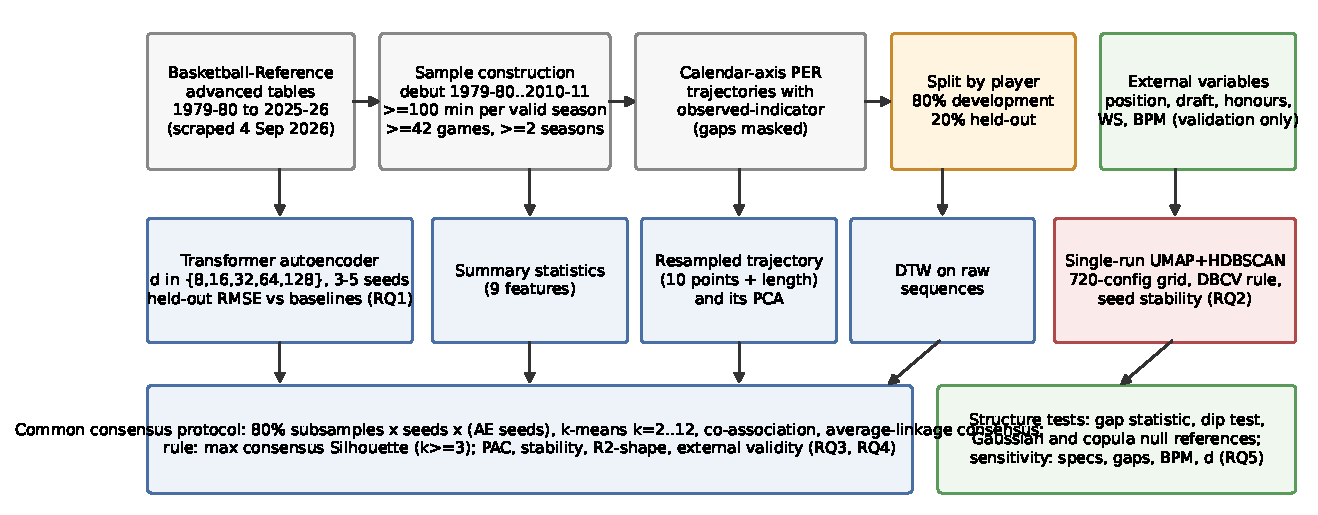
\includegraphics[width=\textwidth]{fig2_pipeline}
\caption{Analytical protocol. Top: data construction and the player-level split. Middle: representations compared on equal terms, and the single-run design of the earlier version, evaluated for reproducibility. Bottom: the common consensus protocol and the tests for discrete structure.}
\label{fig:pipeline}
\end{figure}

\subsection{Transformer autoencoder (RQ1)}\label{sec:ae}

Let $x_i=(x_{i,1},\dots,x_{i,T_i})$ be the standardised PER sequence of player $i$ and $m_{i,t}\in\{0,1\}$ the observed-indicator. Each season is embedded as a token $\bm{u}_{i,t}=\bm{W}_{\mathrm{in}}[x_{i,t}m_{i,t},\,m_{i,t}]^{\top}+\bm{p}_t$, with $\bm{p}_t$ a learned positional embedding. A learned classification token $\bm{u}_{i,0}$ is prepended and the sequence is processed by a Transformer encoder \citep{vaswani2017} with a key-padding mask that removes unobserved and padded positions from attention. The latent code is a linear projection of the final state of the classification token,
\begin{equation}
\bm{z}_i=\bm{W}_z\,\mathrm{Enc}(\bm{u}_{i,0},\dots,\bm{u}_{i,T})_0\in\mathbb{R}^{d},
\label{eq:latent}
\end{equation}
so that the latent dimensionality $d$ is decoupled from the model width. The decoder is a Transformer decoder whose queries are learned positional embeddings $\bm{q}_t$ attending through cross-attention to the single memory vector $\bm{W}_m\bm{z}_i$; a linear read-out gives $\hat{x}_{i,t}$. Training minimises the masked mean-squared error
\begin{equation}
\mathcal{L}=\frac{\sum_{i}\sum_{t=1}^{T} m_{i,t}\,(x_{i,t}-\hat{x}_{i,t})^{2}}{\sum_{i}\sum_{t=1}^{T} m_{i,t}},
\label{eq:loss}
\end{equation}
in which gaps and padding contribute nothing; no cluster information enters training. Table~\ref{tab:aeconfig} lists every architectural and optimisation setting. Latent dimensionalities $d\in\{8,16,32,64,128\}$ were trained with three seeds each ($d=64$ with five); the seed governs initialisation and mini-batch order, and deterministic algorithms were enforced. Held-out RMSE in PER units is compared with three baselines on the same observations: the development-set global mean, each player's own career mean and a player-specific least-squares linear trend. The prespecified criterion for retaining the autoencoder is a held-out RMSE below that of the linear trend.

\begin{table}[t]\centering\small
\caption{Transformer autoencoder: architecture, initialisation, optimisation and validation settings.}
\label{tab:aeconfig}
\begin{tabular}{ll}\toprule
Component & Setting \\ \midrule
Input per season & $[x_{i,t}m_{i,t},\,m_{i,t}]$ (standardised PER, observed indicator) \\
Model width / heads / feed-forward & 64 / 4 / 128 \\
Encoder / decoder layers & 2 / 2 (post-norm, ReLU, dropout 0.1) \\
Positional encoding & learned, season index (encoder) and output position (decoder) \\
Latent dimensionality $d$ & 8, 16, 32, 64, 128 (linear projection of the CLS state) \\
Initialisation & Xavier-uniform weights, zero biases, CLS $\sim\mathcal N(0,0.02^2)$ \\
Loss & masked MSE, Eq.~\eqref{eq:loss} \\
Optimiser & AdamW, learning rate $10^{-3}$, weight decay $10^{-4}$ \\
Batch size / gradient clipping & 64 / global norm 1.0 \\
Schedule & halve learning rate after 15 epochs without validation improvement \\
Epochs / early stopping & at most 400; patience 40 on held-out masked MSE; best epoch restored \\
Data split & 80/20 by player, stratified by career-length tertile, split seed 2026 \\
Seeds & 0--4 ($d=64$), 0--2 (other $d$); deterministic algorithms enforced \\
Parameters & 179,073 ($d=64$) \\
Hardware / time & 2 CPU cores; 8 min per model ($d=64$) \\
\bottomrule\end{tabular}
\end{table}

\subsection{Single-run UMAP+HDBSCAN and its reproducibility (RQ2)}\label{sec:singlerun}

The design of the earlier version, standardisation of the latent codes, UMAP \citep{mcinnes2018} and HDBSCAN \citep{campello2013,mcinnes2017hdbscan}, was re-implemented with a full grid (UMAP dimension $\{2,3,5,10\}$, neighbours $\{10,15,20,30,50\}$, minimum distance $\{0,0.1\}$; HDBSCAN minimum cluster size $\{15,20,25,30,40,50\}$, minimum samples $\{5,10,15\}$; \nGrid{} configurations, Euclidean distance, excess-of-mass extraction), evaluated on the development set only. Three selection rules were compared: (a) the prespecified rule, maximum DBCV \citep{moulavi2014} subject to at most 25\% noise and at least three clusters; (b) maximum Silhouette under the same constraints; (c) the composite score of the earlier version (Silhouette 30\%, noise share 30\%, capped Calinski--Harabasz 20\%, a step function of the number of clusters 20\%). Selected configurations were applied to the held-out players with UMAP's transform and HDBSCAN's approximate prediction, and refitted on all players. Reproducibility was measured directly: for four representative configurations the pipeline was rerun with ten UMAP random states for each of three autoencoder seeds, with excess-of-mass and leaf extraction, and every pair of runs was compared by the adjusted Rand index \citep[ARI;][]{hubert1985}, recording also the number of clusters, the noise share and the size of the largest cluster.

\subsection{Consensus clustering (RQ3)}\label{sec:consensus}

Because single runs proved irreproducible, the reported partitions are resampling-based consensus partitions \citep{monti2003,fred2005}. An ensemble member is an autoencoder seed (five for $d=64$), a random 80\% subsample of players and a random state; for each member and each $k\in\{2,\dots,12\}$ the subsample is partitioned by $k$-means (five initialisations) in the standardised latent space or, in the UMAP variant, in a five-dimensional UMAP embedding refitted on the subsample. With \nMembersAe{} members for the five-seed autoencoder ensemble and \nMembersSumm{} for single-embedding representations, the co-association matrix $C_k$ records for every pair of players the share of members containing both in which they were assigned together; the consensus partition for a given $k$ is the average-linkage agglomeration of $1-C_k$ into $k$ groups. Each $k$ is described by PAC, the share of pairs with $0.1<C_k<0.9$ \citep{senbabaoglu2014}, and by the consensus Silhouette on the distance $1-C_k$. The rule for $k$ selects the $k\ge3$ that maximises the consensus Silhouette. We had initially specified the PAC minimum; PAC decreased almost monotonically in $k$ for every representation (Appendix~\ref{app:k}) and could not select $k$, so the rule was changed before any cluster profile was examined, and both curves are reported. A player's stability is the mean co-association with the other members of its consensus cluster; players below 0.5 are reported as unstable. The same protocol with HDBSCAN in place of $k$-means was also run.

\subsection{Baseline representations and common criteria (RQ4)}\label{sec:baselines}

The protocol was applied unchanged to (i) nine summary statistics (career mean, peak, standard deviation, valid seasons, span, linear slope, first and last season PER, relative position of the peak, share of seasons at or above 15), standardised; (ii) the trajectory resampled by linear interpolation onto ten equally spaced points of normalised career time plus log career length, standardised (``resampled''); (iii) its first six principal components (\pcaVar\% of variance); (iv) $k$-means with dynamic time warping \citep{sakoe1978,petitjean2011,tavenard2020} on the variable-length standardised sequences (``DTW''); and (v) Ward linkage on the summary statistics. Every partition is scored on the same criteria: reproducibility (PAC, consensus Silhouette, share of stable players); trajectory-shape homogeneity, the share of variance of the resampled-trajectory matrix explained by cluster membership, $R^2_{\mathrm{shape}}=1-\mathrm{SS}_{\mathrm{within}}/\mathrm{SS}_{\mathrm{total}}$, a space no method optimised directly; and external validity, Cram\'er's $V$ and adjusted mutual information \citep{vinh2010} with position, draft category, All-Star and All-NBA selection, and the Kruskal--Wallis $\varepsilon^2$ \citep{kruskal1952,tomczak2014} for career WS, mean BPM and career games. Internal indices in each method's own space are reported in Appendix~\ref{app:internal} but not used across representations.

\subsection{Tests for discrete structure and a continuous description}\label{sec:structure_methods}

Reproducibility is necessary but not sufficient for the existence of types, because $k$-means partitions even a unimodal cloud stably \citep{senbabaoglu2014}. Four analyses address this. (i) The gap statistic \citep{tibshirani2001} compares $\log W_k$, the within-cluster dispersion of $k$-means, with its expectation under reference data without structure, for $k=1,\dots,12$ and $B=20$ draws from a uniform distribution over the principal-component bounding box and from a multivariate normal with the sample covariance; $k$ is chosen by the rule of \citet{tibshirani2001}. (ii) Hartigan's dip test of unimodality \citep{hartigan1985} is applied to the first three principal components of each representation and to individual summary statistics. (iii) The consensus protocol itself is applied to three draws from a multivariate normal with the mean and covariance of the real features and to three draws from a Gaussian copula that preserves every real marginal and the rank correlations but imposes a unimodal dependence structure. (iv) To separate level from shape, the protocol and the dip test are applied to a shape-only representation (each resampled trajectory minus its own mean, length excluded), the representation closest to the functional-data analyses of \citet{wakim2014}. As a constructive alternative to types, principal components of the resampled trajectory in PER units are related to level, slope, peak timing and length, and a linear discriminant on these coordinates is used to measure how much of the typology they reproduce.

\subsection{Sensitivity, labelling and software (RQ5)}\label{sec:sens_methods}

The full pipeline was repeated for latent dimensionalities 8, 16, 32 and 128, for a single autoencoder seed, unstandardised codes and a UMAP stage; and both the autoencoder pipeline and the summary-statistic typology were repeated for the six alternative sample specifications of Table~\ref{tab:flow}, for gap deletion and for BPM in place of PER. Agreement with the primary partition is measured by ARI on common players. Cluster labels follow a rule fixed before the results were examined: a level term from the cluster median of career-mean PER (below 12, 12--18, above 18), a duration term from the median of valid seasons (at most 4, 5--9, at least 10) and a shape qualifier only when the median slope exceeds 0.25 PER per season in absolute value. Named players are the three nearest to each cluster medoid, plus well-known players whose membership is discussed only as illustration. Analyses used Python 3.11 with PyTorch \citep{paszke2019}, scikit-learn \citep{pedregosa2011}, umap-learn, hdbscan \citep{mcinnes2017hdbscan} and tslearn \citep{tavenard2020} on two CPU cores; all seeds are fixed in the released code, which also regenerates every number in this paper from the result files.

\section{Results}\label{sec:results}

\subsection{Sample and reconstruction (RQ1)}\label{sec:res_recon}

The primary sample contains \nPlayers{} players and \nObs{} valid PER observations (Table~\ref{tab:flow}); the median career has \medianSeasons{} valid seasons (mean \meanSeasons), the longest 23, and positions are balanced (318 to 349 players per modal position). Figure~\ref{fig:examples} shows four careers that illustrate the heterogeneity the analysis must accommodate, including gaps.

\begin{table}[t]\centering\small
\caption{Construction of the analysis sample under the primary and alternative specifications. Players enter if their first NBA season is in the debut window; ``career games'' and ``valid seasons'' are the successive restrictions; the last column counts season observations that enter the loss.}
\label{tab:flow}
\resizebox{\textwidth}{!}{\begin{tabular}{lrrrr}\toprule
Specification & Debut in window & Career games & Valid seasons & PER observations \\ \midrule
Primary & 2,381 & 1,833 & 1,676 & 13,193 \\
No minutes threshold, PER$>$45 removed (2025 version) & 2,381 & 1,833 & 1,749 & 14,128 \\
250-minute threshold & 2,381 & 1,833 & 1,544 & 12,168 \\
At least 3 valid seasons & 2,381 & 1,833 & 1,444 & 12,729 \\
No career-games restriction & 2,381 & 2,381 & 1,685 & 13,211 \\
Debut 1979--80 to 2005--06 & 2,051 & 1,577 & 1,437 & 11,254 \\
\bottomrule\end{tabular}}
\end{table}

\begin{figure}[t]\centering
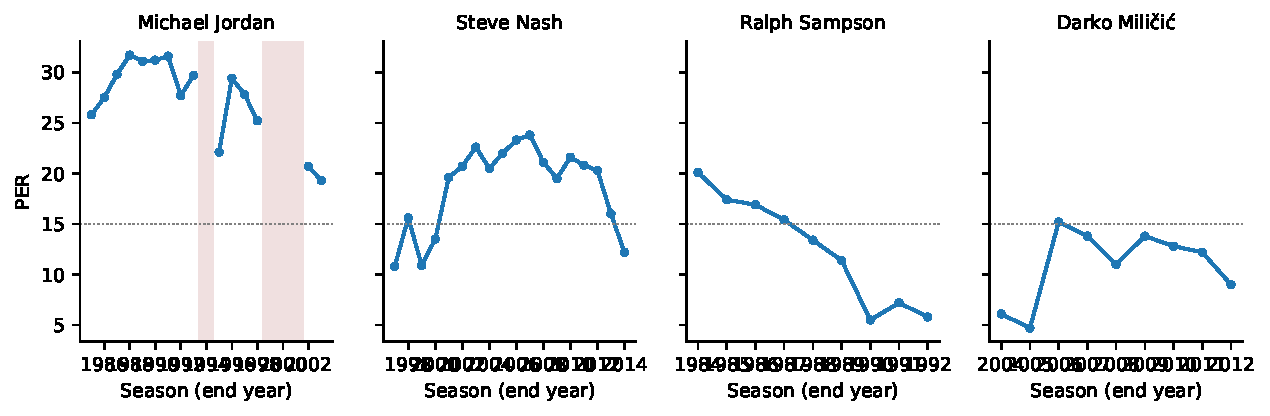
\includegraphics[width=\textwidth]{fig1_examples}
\caption{Four PER careers on the calendar axis. Shaded seasons are gaps (fewer than 100 minutes); the dotted line is the league average of 15. Michael Jordan's two retirements produce gaps that are masked rather than interpolated.}
\label{fig:examples}
\end{figure}

The autoencoder with $d=64$ reaches a held-out RMSE of \rmseHeld{} PER points (SD over five seeds \rmseHeldSd; training RMSE \rmseTrain), against \rmseLinear{} for a player-specific linear trend, \rmsePlayerMean{} for the player's own mean and \rmseGlobal{} for the global mean (Table~\ref{tab:recon}, Figure~\ref{fig:recon}); the prespecified criterion is met by a wide margin, and a 70/10/20 split gives \rmseTestThreeWay{} (Appendix~\ref{app:training}). Error falls steeply from $d=8$ (\rmseHeldEight) to $d=32$ (\rmseHeldThirtytwo) and is flat thereafter (\rmseHeldOneTwoEight{} at $d=128$). Because no career exceeds \maxSpan{} seasons, a code of 32 or more dimensions can store the sequence itself; the plateau shows that the model does so almost losslessly. This matters for clustering: a near-lossless code preserves all the idiosyncratic detail of a career, including detail shared with no other career.

\begin{table}[t]\centering\small
\caption{Reconstruction RMSE in PER units on the development (train) and held-out players, by latent dimensionality, with three baselines evaluated on the same held-out observations.}
\label{tab:recon}
\resizebox{\textwidth}{!}{\begin{tabular}{lcccc}\toprule
Model & Seeds & Train RMSE & Held-out RMSE (SD over seeds) & Best epoch \\ \midrule
Transformer autoencoder, $d=8$ & 3 & 0.88 & 1.23 (0.07) & 309 \\
Transformer autoencoder, $d=16$ & 3 & 0.61 & 0.95 (0.20) & 353 \\
Transformer autoencoder, $d=32$ & 3 & 0.47 & 0.80 (0.08) & 367 \\
Transformer autoencoder, $d=64$ & 10 & 0.43 & 0.74 (0.06) & 361 \\
Transformer autoencoder, $d=128$ & 3 & 0.41 & 0.74 (0.02) & 358 \\
\midrule Player-specific linear trend (2 parameters) & -- & -- & 2.24 & -- \\
Player mean & -- & -- & 2.76 & -- \\
Global mean & -- & -- & 4.35 & -- \\
\bottomrule\end{tabular}}
\end{table}

\begin{figure}[t]\centering
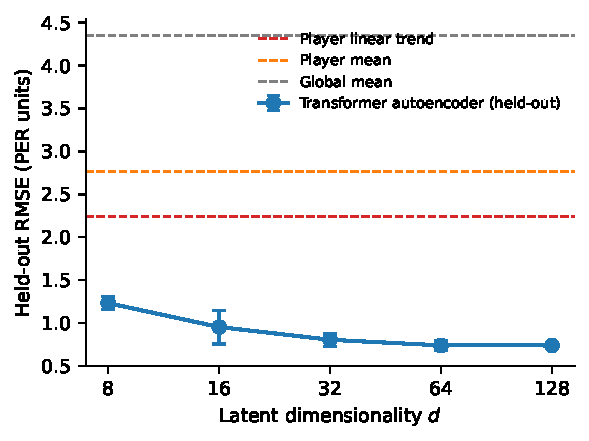
\includegraphics[width=0.55\textwidth]{fig3_reconstruction}
\caption{Held-out reconstruction RMSE of the Transformer autoencoder as a function of latent dimensionality (mean and SD over seeds), with the three baselines.}
\label{fig:recon}
\end{figure}

\subsection{A single UMAP+HDBSCAN run is not reproducible (RQ2)}\label{sec:res_single}

Over the \nGrid{} grid configurations, HDBSCAN returned between \gridKmin{} and \gridKmax{} clusters. The three selection rules chose three different solutions (Appendix Table~\ref{tab:selection}): the DBCV rule a ten-dimensional embedding with \selDbcvKdev{} clusters on the development set, \selDbcvKho{} on the held-out players and \selDbcvKall{} when refitted on all players; the Silhouette rule and the composite rule of the earlier version two-dimensional embeddings with \selSilKdev{} and \selCompKdev{} clusters, which became \selSilKall{} and \selCompKall{} on refitting, with \selSilNoiseho\% and \selCompNoiseho\% of held-out players unassigned. The selected solution depends more on the rule and the sample than on the data.

Figure~\ref{fig:single} (details in Appendix Table~\ref{tab:stability}) measures reproducibility directly. Holding the autoencoder fixed and changing only the UMAP random state, the mean pairwise ARI between runs ranged from \ariSingleMin{} to \ariSingleMax{} across configurations and extraction methods, never reaching the criterion of 0.80, and the number of clusters within a configuration varied between \kSingleMin{} and \kSingleMax{}. With excess-of-mass extraction the largest cluster contained between \bigShareEomMin\% and \bigShareEomMax\% of players on average, and it was this cluster whose subdivision changed from run to run; leaf extraction produced more and smaller clusters at the cost of \noiseLeafMean\% noise. Changing the autoencoder seed at a fixed UMAP seed gave mean ARIs between \ariAeSeedsMin{} and \ariAeSeedsMax{}. RQ2 is answered in the negative: the design of the earlier version, and by extension its nineteen-cluster solution, does not describe a reproducible partition. The instability has two sources, the stochastic embedding and, more fundamentally, the dependence of the learned latent geometry on the training seed.

\begin{figure}[t]\centering
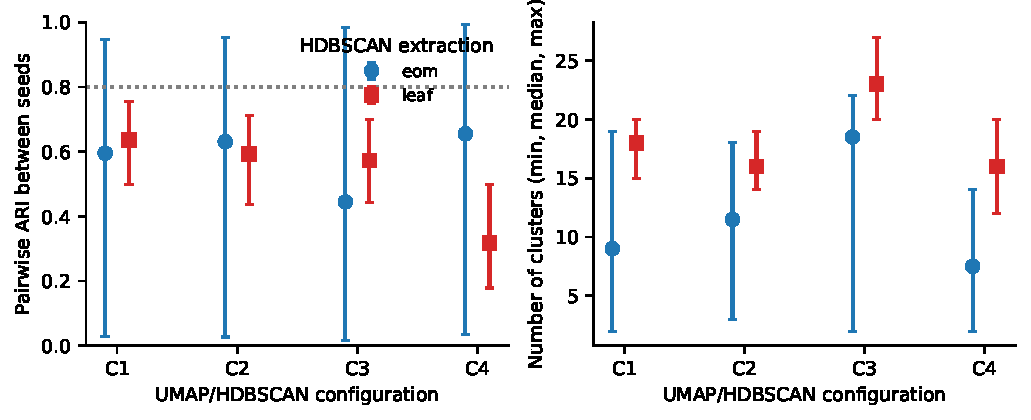
\includegraphics[width=0.9\textwidth]{fig4_single_run}
\caption{Reproducibility of single UMAP+HDBSCAN runs across ten UMAP random states (three autoencoder seeds each) for four configurations (C1--C4, Appendix Table~\ref{tab:stability}) and two extraction methods. Left: pairwise ARI (mean, with range); the dotted line is the prespecified criterion. Right: number of clusters (median, with range).}
\label{fig:single}
\end{figure}

\subsection{Consensus clustering of the learned representation (RQ3)}\label{sec:res_consensus}

With all five autoencoder seeds in the ensemble (\nMembersAe{} members), the consensus Silhouette of the learned representation peaks at $k=\aeAllK$ (\aeAllSil, PAC \aeAllPac) and declines thereafter (\aeAllSilTwelve{} at $k=12$); at $k=8$ only \aeAllStableEight\% of players have a stability score of 0.5 or more (Figure~\ref{fig:consensus}, Table~\ref{tab:baselines}). When the ensemble is restricted to a single autoencoder seed, so that only subsampling varies, the consensus is far tighter (\aeSeedZeroSil{} at $k=3$, \aeSeedZeroSilEight{} at $k=8$, \aeSeedZeroStableEight\% stable). The two ensembles differ only in the inclusion of independently trained encoders, so the dominant source of irreproducibility is the training seed: two runs of the same model on the same data learn latent geometries whose partitions agree only moderately (ARI \ariASeedZero{} between the single-seed and the five-seed consensus). Leaving the latent coordinates unstandardised (\aeNostdSil{} at $k=3$), inserting UMAP before $k$-means (\aeUmapSil{} at $k=3$ but \aeUmapSilEight{} at $k=8$) or embedding HDBSCAN itself in the consensus (PAC \aeHdbPac, \aeHdbStable\% stable) does not change this, and neither does latent dimensionality (coarse consensus Silhouette \aeEightSil{} to \aeOneTwoEightSil{} for $d=8$ to $128$; Table~\ref{tab:sensitivity}a). For the learned representation, a three-group coarse structure, essentially level and length of career, is reproducible across seeds; anything finer is not.

\begin{figure}[t]\centering
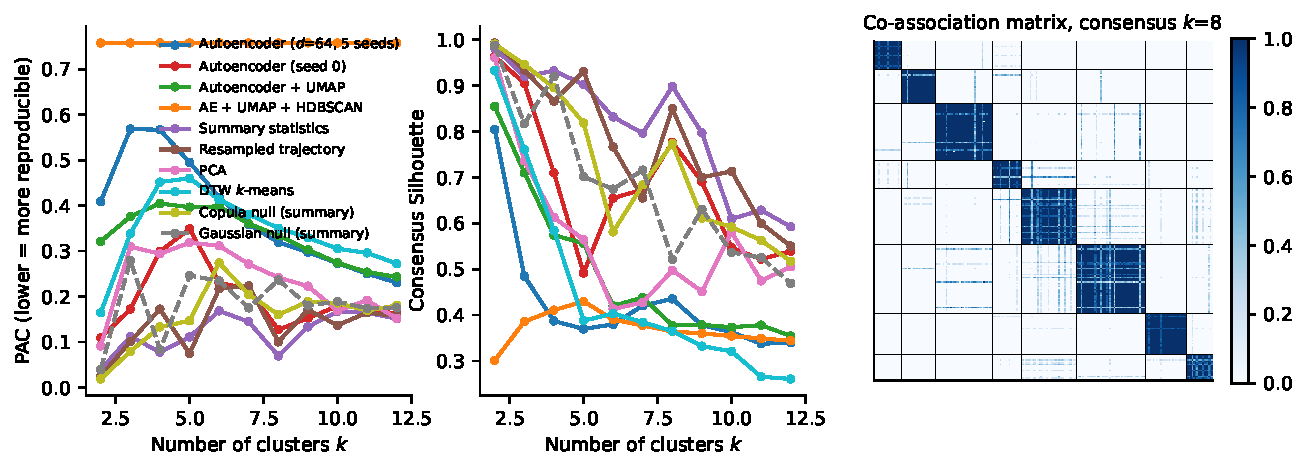
\includegraphics[width=\textwidth]{fig5_consensus}
\caption{Consensus diagnostics by number of clusters $k$ for the main representations and two structureless references (left: PAC; centre: consensus Silhouette), and the co-association matrix of the summary-statistic representation ordered by the $k=8$ consensus partition (right; black lines separate the types).}
\label{fig:consensus}
\end{figure}

\subsection{Learned representation versus baselines (RQ4)}\label{sec:res_baselines}

Table~\ref{tab:baselines} compares every representation under the same protocol. The nine summary statistics and the resampled trajectory are markedly more reproducible than any variant of the learned representation: at $k=8$ their consensus Silhouettes are \summSilEight{} and \rawSilEight{} against \aeAllSilEight, with \summStableEight\% and \rawStableEight\% of players stable against \aeAllStableEight\%; they explain more trajectory-shape variance ($R^2_{\mathrm{shape}}$ \summRsqEight{} and \rawRsqEight{} against \aeAllRsqEight) and are at least as strongly associated with All-Star selection and career Win Shares. Ward linkage on the summary statistics (\summWardSilEight) and PCA of the resampled trajectory (\pcaSilEight) are intermediate. DTW $k$-means on the raw sequences, the most direct classical competitor, \dtwSentence

Reproducibility within a representation does not translate into agreement between representations: the $k=8$ partitions of the summary statistics and the resampled trajectory agree at ARI \xSummaryRaw, and every pairing involving the autoencoder lies between \xMin{} and \xMax{} (Appendix Table~\ref{tab:crossrep}). Each representation partitions the same players reproducibly but differently. RQ4 is answered in the negative for the learned representation, and the disagreement raises the question addressed next: whether \emph{any} of these partitions reflects discrete structure.

\begin{table}[t]\centering\scriptsize
\caption{All representations under the same consensus protocol. Sil.$_C$ = consensus Silhouette; PAC = proportion of ambiguous pairs; Stable \% = share of players with stability $\ge 0.5$; $R^2_{\mathrm{shape}}$ = share of resampled-trajectory variance explained by cluster membership; $V_{\mathrm{AS}}$ = Cram\'er's $V$ with All-Star selection; $\varepsilon^2_{\mathrm{WS}}$ = Kruskal--Wallis effect size for career Win Shares. Left block: $k$ selected by the rule; right block: all representations at $k=8$.}
\label{tab:baselines}
\resizebox{\textwidth}{!}{\begin{tabular}{lcccccccccccc}\toprule
 & & \multicolumn{5}{c}{Selected $k$ (rule)} & \multicolumn{6}{c}{Matched comparison at $k=8$} \\ \cmidrule(lr){3-7}\cmidrule(lr){8-13}
Representation & Members & $k$ & Sil.$_C$ & PAC & Stable \% & $R^2_{\mathrm{shape}}$ & Sil.$_C$ & PAC & Stable \% & $R^2_{\mathrm{shape}}$ & $V_{\mathrm{AS}}$ & $\varepsilon^2_{\mathrm{WS}}$ \\ \midrule
Autoencoder $d=64$, 5 seeds (latent space) & 40 & 3 & 0.48 & 0.57 & 80 & 0.37 & 0.44 & 0.32 & 67 & 0.50 & 0.61 & 0.65 \\
Autoencoder $d=64$, seed 0 only & 20 & 3 & 0.90 & 0.17 & 100 & 0.41 & 0.78 & 0.13 & 95 & 0.50 & 0.56 & 0.60 \\
Autoencoder $d=64$, 5 seeds, unstandardised & 40 & 3 & 0.56 & 0.50 & 94 & 0.46 & 0.45 & 0.31 & 70 & 0.57 & 0.63 & 0.67 \\
Autoencoder $d=64$, 5 seeds + UMAP (5-D) & 40 & 3 & 0.71 & 0.38 & 95 & 0.24 & 0.38 & 0.33 & 49 & 0.29 & 0.40 & 0.70 \\
Autoencoder + UMAP + HDBSCAN (consensus) & 40 & 5 & 0.43 & 0.76 & 66 & 0.18 & 0.36 & 0.76 & 66 & 0.18 & 0.29 & 0.54 \\
Autoencoder $d=8$, 3 seeds & 24 & 3 & 0.50 & 0.55 & 90 & 0.40 & 0.34 & 0.35 & 46 & 0.48 & 0.60 & 0.58 \\
Autoencoder $d=16$, 3 seeds & 24 & 4 & 0.57 & 0.41 & 86 & 0.38 & 0.35 & 0.32 & 53 & 0.48 & 0.63 & 0.61 \\
Autoencoder $d=32$, 3 seeds & 24 & 3 & 0.62 & 0.46 & 91 & 0.39 & 0.37 & 0.33 & 50 & 0.49 & 0.62 & 0.64 \\
Autoencoder $d=128$, 3 seeds & 24 & 3 & 0.70 & 0.39 & 92 & 0.39 & 0.49 & 0.29 & 71 & 0.46 & 0.62 & 0.63 \\
Summary statistics, $k$-means & 8 & 4 & 0.93 & 0.08 & 99 & 0.47 & 0.90 & 0.07 & 99 & 0.60 & 0.68 & 0.75 \\
Summary statistics, Ward & 8 & 3 & 0.49 & 0.62 & 96 & 0.42 & 0.47 & 0.33 & 81 & 0.55 & 0.66 & 0.73 \\
Resampled trajectory, $k$-means & 8 & 3 & 0.93 & 0.10 & 99 & 0.57 & 0.85 & 0.10 & 97 & 0.72 & 0.65 & 0.71 \\
PCA of resampled trajectory, $k$-means & 8 & 3 & 0.74 & 0.31 & 94 & 0.14 & 0.50 & 0.24 & 80 & 0.34 & 0.48 & 0.55 \\
DTW $k$-means on sequences & 8 & 3 & 0.76 & 0.34 & 97 & 0.53 & 0.36 & 0.35 & 70 & 0.66 & 0.64 & 0.51 \\
\bottomrule\end{tabular}}
\end{table}

\subsection{Discrete types or a continuum?}\label{sec:res_structure}

Three tests were applied (Table~\ref{tab:structure}). The gap statistic \citep{tibshirani2001} grows monotonically in $k$ against a uniform reference for every representation, the signature of a continuous correlated cloud, and is close to zero for every $k$ against a multivariate-normal reference with the same covariance (maximum \gapSummNormalMax{} for the summary statistics, \gapRawNormalMax{} for the resampled trajectory, \gapAeNormalMax{} for the learned representation); the gap rule selects $k=1$ for all three. Hartigan's dip test \citep{hartigan1985} finds no multimodality on the first three principal components of any representation ($p$ between \dipPmin{} and \dipPmax); among the summary statistics only the number of seasons, a discrete count with a long right tail, rejects unimodality. Finally, the consensus protocol was applied to structureless references \citep{senbabaoglu2014}. \nullSentence

The three tests agree: the reproducible partitions of Section~\ref{sec:res_baselines} are reproducible segmentations of a continuum, not recoveries of discrete career types.

\begin{table}[t]\centering\small
\caption{Tests for discrete structure. Gap statistic: maximum over $k=2,\dots,12$ against a multivariate-normal reference with the sample covariance and the $k$ selected by the gap rule. Dip test: $p$-values of Hartigan's test on the first three principal components. Null consensus: mean consensus Silhouette over three simulated datasets at $k=4$ and $k=8$ for a multivariate-normal reference and for a Gaussian copula with the real marginals. $^a$Gap and dip statistics for the autoencoder are computed on the seed-0 latent space; consensus values are for the five-seed ensemble.}
\label{tab:structure}
\resizebox{\textwidth}{!}{\begin{tabular}{lcccccc}\toprule
 & \multicolumn{2}{c}{Gap statistic (normal ref.)} & Dip test & \multicolumn{3}{c}{Consensus Silhouette, $k=4$ / $k=8$} \\ \cmidrule(lr){2-3}\cmidrule(lr){4-4}\cmidrule(lr){5-7}
Representation & max gap & selected $k$ & min $p$ (PC1--3) & Real data & Gaussian null & Copula null \\ \midrule
Summary statistics & 0.16 & 1 & 0.71 & 0.93 / 0.90 & 0.93 / 0.56 & 0.90 / 0.75 \\
Resampled trajectory & 0.01 & 1 & 0.99 & 0.87 / 0.85 & 0.93 / 0.63 & 0.87 / 0.66 \\
Autoencoder $d=64$, 5 seeds$^a$ & 0.11 & 1 & 0.93 & 0.39 / 0.44 & -- / -- & -- / -- \\
\bottomrule\end{tabular}}
\end{table}

\subsection{A continuous description of careers}\label{sec:res_continuous}

If careers form a continuum, the natural summary is a small set of continuous coordinates. Principal components of the resampled trajectory (ten points of normalised career time, PER units) provide one (Figure~\ref{fig:continuous}). The first component (\pcOneVar\% of variance) is career level: $r=\pcOneMean$ with career-mean PER, \pcOnePeak{} with peak PER, \pcOneWs{} with career Win Shares. The second (\pcTwoVar\%) is the tilt of the career, rising versus declining: uncorrelated with level ($|r|=\pcTwoMean$), $r=\pcTwoSlope$ with the linear slope and \pcTwoPeakpos{} with the relative position of the peak. Career length is a third, separate coordinate. A linear classifier on level, tilt and log length recovers the eight fine types of Section~\ref{sec:profiles} with \ldaAccThree\% cross-validated accuracy (\ldaAccTwo\% from level and tilt alone), so most of the typology is a discretisation of these three coordinates: the types are contiguous bands in the level--tilt plane with no empty regions between them, and the density of players in that plane is a single unimodal cloud.

The same holds when level is removed. On the shape-only representation (each trajectory minus its own mean), the consensus protocol is again highly reproducible ($k=\shapeK$, consensus Silhouette \shapeSil) and returns the early, middle and late peakers of \citet{wakim2014} (Table~\ref{tab:shape}; median peak position \shapePpA, \shapePpB{} and \shapePpC{} of the career). But the dip test finds no multimodality in the shape components ($p\ge\shapeDipPmin$) or in the slope ($p=\dipSlopeP$), and the shape groups differ strongly in career length (median \shapeSeasA, \shapeSeasB{} and \shapeSeasC{} seasons; $\varepsilon^2=\shapeLenEps$), as expected when short careers are stretched onto normalised time. Peak timing is a continuous property of this population: \peakFirstThird\% of players peak in the first third of their career and \peakLastThird\% in the last third, with no gap in between.

\begin{figure}[t]\centering
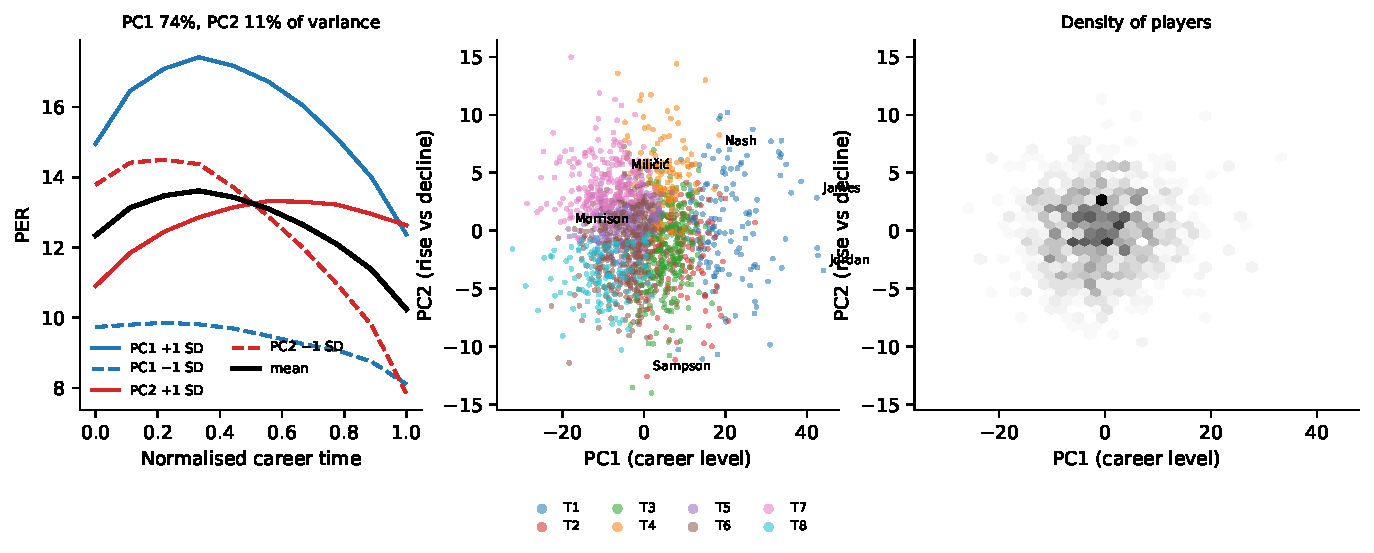
\includegraphics[width=\textwidth]{fig9_continuous}
\caption{A continuous description. Left: mean resampled PER trajectory and the effect of one standard deviation of the first two principal components (PC1, career level; PC2, rise versus decline). Centre: players in the PC1--PC2 plane coloured by fine type, with selected players labelled. Right: density of players in the same plane.}
\label{fig:continuous}
\end{figure}

\begin{table}[t]\centering\small
\caption{Shape-only consensus groups ($k=\shapeK$; resampled trajectory minus the player's own mean, length excluded), ordered by median peak position; medians per group.}
\label{tab:shape}
\begin{tabular}{lcccccccc}\toprule
Shape group & $n$ & Peak position & Slope & First-season PER & Last-season PER & Mean PER & Seasons & All-Star \% \\ \midrule
S1 & 613 & 0.33 & -0.69 & 14.0 & 8.9 & 12.5 & 8 & 17 \\
S2 & 400 & 0.50 & -0.19 & 11.8 & 9.9 & 13.9 & 11 & 30 \\
S3 & 663 & 0.70 & +0.05 & 10.9 & 11.3 & 11.5 & 4 & 3 \\
\bottomrule\end{tabular}
\end{table}

\subsection{A descriptive typology of the continuum}\label{sec:profiles}

Continuous coordinates are the more faithful summary, but a reproducible segmentation remains useful for description, provided it is not mistaken for a discovery of natural kinds. We therefore also report the consensus partition of the most reproducible representation, the summary statistics, at $k=8$ (Table~\ref{tab:profiles8}, Figure~\ref{fig:profiles}), where the consensus Silhouette is \summSilEight{} and \summStableEight\% of players are stable; the rule-selected $k=\mainK$ solution, in which the eight types nest imperfectly (\nestingPurity\% purity), is given in Appendix~\ref{app:nesting}. Labels follow the rule of Section~\ref{sec:methods}. The long-career groups split by level into a high-PER group (T1: \eightNA{} players, median PER \eightPerA, \eightASA\% All-Stars), a moderate-PER group (T3) and a low-PER group (T6); two medium-length groups differ in direction (T2, early peak then decline; T4, late rise); and the short-career groups are flat-declining (T5), rising (T7) and steeply declining (T8). Median stability is at least \eightStabMin{} in every type. Named players illustrate rather than validate: Michael Jordan, Kobe Bryant, Larry Bird, Stephen Curry and LeBron James are all in \typeJordan, as are Isiah Thomas and Steve Nash; Ralph Sampson is in \typeSampson, Darko Mili\v{c}i\'c in \typeMilicic{} and Adam Morrison in \typeMorrison. The players nearest each type's medoid (Table~\ref{tab:profiles8}) are, by construction, not stars, and represent better what a type typically contains.

\begin{table}[t]\centering\scriptsize
\caption{Fine types ($k=8$) of the summary-statistic consensus, ordered by median career-mean PER and length. Labels follow the fixed rule (level: $>18$ high, 12--18 moderate, $<12$ low; duration: $\ge10$ long, 5--9 medium, $\le4$ short; slope qualifier if $|\text{slope}|>0.25$ PER per season).}
\label{tab:profiles8}
\resizebox{\textwidth}{!}{\begin{tabular}{lcccccccclp{3.6cm}}\toprule
Type & $n$ & Stability & Mean PER & Peak PER & Seasons & Slope & All-Star \% & Career WS & Label (rule) & Nearest to medoid \\ \midrule
T1 & 138 & 0.98 & 18.5 & 23.6 & 14 & -0.23 & 86 & 89.6 & high-PER, long career & Shawn Kemp, Paul George, Sam Cassell \\
T2 & 166 & 0.95 & 15.1 & 18.1 & 6 & -1.02 & 19 & 16.8 & moderate-PER, medium career, declining & Lawrence Funderburke, Edgar Jones, Lewis Lloyd \\
T3 & 283 & 0.96 & 14.2 & 18.4 & 13 & -0.30 & 28 & 49.1 & moderate-PER, long career, declining & Brendan Haywood, Brad Davis, Jeff Malone \\
T4 & 141 & 0.96 & 13.8 & 16.9 & 7 & +0.25 & 6 & 13.4 & moderate-PER, medium career, rising & Marty Conlon, Will Bynum, Darius Miles \\
T5 & 276 & 0.95 & 11.2 & 13.0 & 4 & -0.40 & 0 & 3.8 & low-PER, short career, declining & Bob Wilkerson, Obinna Ekezie, Tom Garrick \\
T6 & 339 & 0.95 & 11.2 & 14.7 & 10 & -0.37 & 1 & 17.1 & low-PER, long career, declining & Dante Cunningham, Brad Lohaus, Kevin Duckworth \\
T7 & 206 & 0.98 & 9.5 & 11.8 & 3 & +0.90 & 0 & 0.8 & low-PER, short career, rising & Scott Roth, Delaney Rudd, Laron Profit \\
T8 & 127 & 0.90 & 9.5 & 12.4 & 3 & -2.90 & 0 & 1.3 & low-PER, short career, declining & Jon Brockman, Chris Welp, Samardo Samuels \\
\bottomrule\end{tabular}}
\end{table}

\begin{figure}[t]\centering
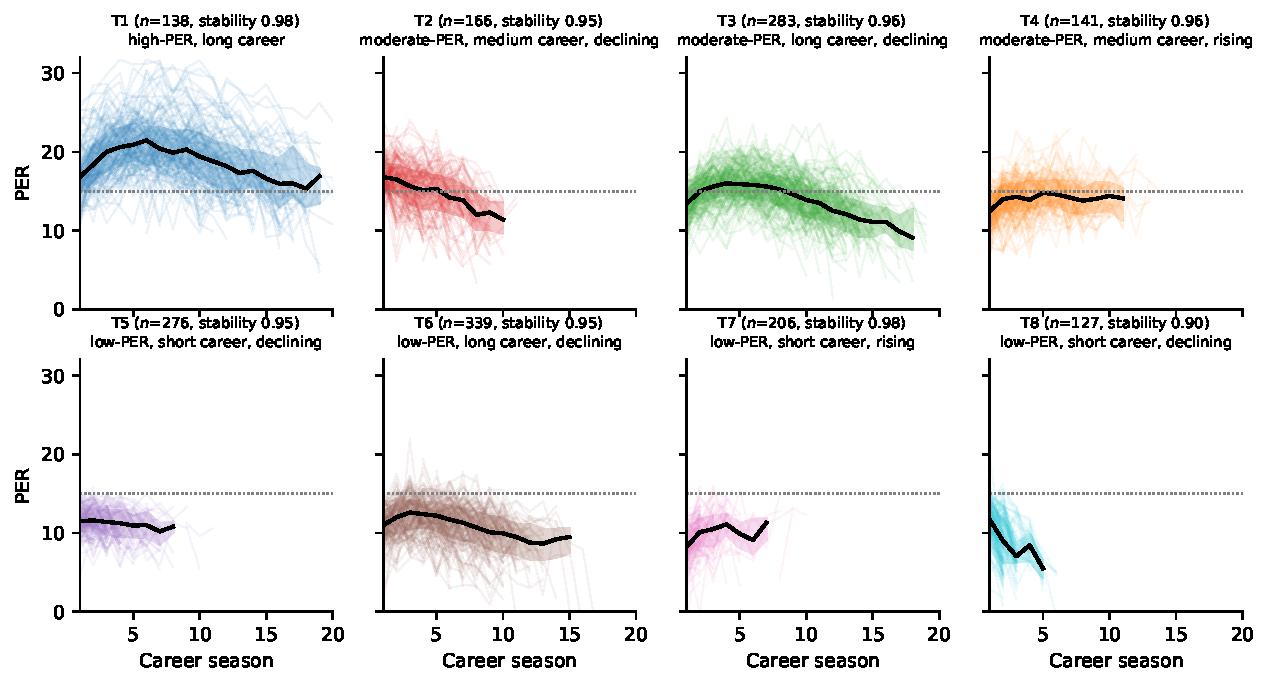
\includegraphics[width=\textwidth]{fig6_profiles}
\caption{PER trajectories of the eight fine types on the career-season axis: individual careers (thin lines, up to 150 per panel), median (black) and interquartile band (shaded), computed at seasons with at least ten observations; $n$ and median stability per type.}
\label{fig:profiles}
\end{figure}

\subsection{External validation (RQ5)}\label{sec:res_external}

Table~\ref{tab:external} relates the eight types to variables that played no part in clustering. Associations with honours and value are large: Cram\'er's $V$ is \VAllStar{} for ever being an All-Star and \VAllNba{} for All-NBA selection; $\varepsilon^2=\epsWs$ for career Win Shares and \epsBpm{} for mean BPM; \eightASA\% of T1 players were All-Stars against at most \eightASmaxOther\% in any other type. The association with draft category is moderate ($V=\VDraft$): \eightLotteryA\% of T1 were lottery picks, whereas the short-career types are dominated by second-round and undrafted players. Position is unrelated to type ($V=\VPos$, $p=\pPos$): the types describe productivity paths, not roles, consistent with \citet{wakim2014}. Because All-Star selection, WS and BPM share inputs with PER, these associations show that the types are not artefacts of the representation, not that they carry information beyond box-score productivity.

\begin{table}[t]\centering\scriptsize
\caption{External variables by fine type. Draft category and position are row percentages; honours are the share of players with at least one selection; WS, BPM and games are medians. Last row: effect sizes over the eight types.}
\label{tab:external}
\resizebox{\textwidth}{!}{\begin{tabular}{lccccccccccc}\toprule
 & \multicolumn{4}{c}{Draft category (\% of type)} & Position & \multicolumn{2}{c}{Honours (\%)} & \multicolumn{3}{c}{Career value (median)} \\ \cmidrule(lr){2-5}\cmidrule(lr){6-6}\cmidrule(lr){7-8}\cmidrule(lr){9-11}
Type & Lottery & 1st rd & 2nd rd & Undrafted & PG/SG/SF/PF/C & All-Star & All-NBA & WS & BPM & Games \\ \midrule
T1 & 71 & 15 & 9 & 5 & 17/15/17/25/26 & 86 & 68 & 89.6 & 1.8 & 968 \\
T2 & 28 & 16 & 17 & 39 & 14/15/22/27/22 & 19 & 6 & 16.8 & -0.7 & 357 \\
T3 & 47 & 29 & 16 & 7 & 25/18/19/22/17 & 28 & 9 & 49.1 & -0.3 & 866 \\
T4 & 26 & 37 & 21 & 16 & 21/18/19/16/25 & 6 & 2 & 13.4 & -1.1 & 396 \\
T5 & 13 & 25 & 33 & 29 & 20/17/19/23/21 & 0 & 0 & 3.8 & -2.7 & 216 \\
T6 & 22 & 31 & 29 & 18 & 19/20/21/19/20 & 1 & 0 & 17.1 & -2.2 & 584 \\
T7 & 12 & 25 & 43 & 20 & 22/27/17/15/20 & 0 & 0 & 0.8 & -3.7 & 134 \\
T8 & 12 & 22 & 32 & 34 & 18/20/24/17/21 & 0 & 0 & 1.3 & -3.9 & 106 \\
\midrule Cram\'er's $V$ / $\varepsilon^2$ & \multicolumn{4}{c}{$V=0.27$} & $V=0.08$ & $V=0.68$ & $V=0.68$ & $\varepsilon^2=0.75$ & $\varepsilon^2=0.54$ & $\varepsilon^2=0.74$ \\
\bottomrule\end{tabular}}
\end{table}

\subsection{Sensitivity analyses (RQ5)}\label{sec:sensitivity}

Table~\ref{tab:sensitivity} reports agreement with the reference partition when one element of the analysis is changed. For the summary-statistic typology (panel b), dropping the games rule and deleting gaps leave the $k=8$ partition essentially unchanged (ARI \ariSEightSummaryNogames{} and \ariSEightSummaryConsecutive), whereas restrictions that remove players change it more (ARI \ariSEightMinRestrict{} to \ariSEightMaxRestrict), partly because the rule then selects $k=3$ rather than $4$ and partly because $k$-means boundaries move when the sample distribution is reshaped. Replacing PER by BPM changes the partition substantially (ARI \ariSEightBpm) although career-mean PER and BPM correlate at $r=\corrPerBpm$: the segmentation is metric-specific. Both patterns are what a continuum implies. For the learned representation (panel a) every change, including changes that alter nothing but the training seed, moves the partition substantially (ARI \ariAMin{} to \ariAMax). Finally, the nineteen-cluster solution of the earlier version, matched by name for \nMatchedOld{} clustered players, has an ARI of \ariOldEight{} with the fine typology and \ariOldAe{} with the learned-representation consensus; it is not recovered by any reproducible analysis.

\begin{table}[t]\centering\small
\caption{Sensitivity of the partitions: ARI with the reference partition on players common to both analyses, at the selected $k$ of each variant and at $k=8$.}
\label{tab:sensitivity}
\resizebox{\textwidth}{!}{\begin{tabular}{lcccc}\toprule
Variant & Common players & Selected $k$ & ARI with reference (selected $k$) & ARI with reference ($k=8$) \\ \midrule
\multicolumn{5}{l}{\textit{(a) Autoencoder pipeline, reference: AE $d$=64, five seeds, $k$-means consensus}} \\
Single AE seed & 1676 & 3 & 0.58 & 0.57 \\
Unstandardised latent & 1676 & 3 & 0.54 & 0.52 \\
UMAP before $k$-means & 1676 & 3 & 0.31 & 0.29 \\
UMAP + HDBSCAN & 1676 & 5 & 0.24 & 0.18 \\
AE $d$=8 & 1676 & 3 & 0.33 & 0.38 \\
AE $d$=16 & 1676 & 4 & 0.29 & 0.40 \\
AE $d$=32 & 1676 & 3 & 0.54 & 0.51 \\
AE $d$=128 & 1676 & 3 & 0.62 & 0.53 \\
2025 restrictions & 1676 & 3 & 0.20 & 0.18 \\
250-minute threshold & 1544 & 3 & 0.35 & 0.29 \\
$\ge$3 seasons & 1444 & 3 & 0.35 & 0.27 \\
No games rule & 1676 & 3 & 0.41 & 0.38 \\
Debut $\le$2005--06 & 1437 & 3 & 0.39 & 0.37 \\
Gaps deleted & 1676 & 3 & 0.62 & 0.38 \\
BPM instead of PER & 1676 & 3 & 0.32 & 0.24 \\
\midrule \multicolumn{5}{l}{\textit{(b) Summary-statistic typology, reference: primary consensus}} \\
2025 restrictions & 1676 & 3 & 0.31 & 0.51 \\
250-minute threshold & 1544 & 3 & 0.48 & 0.59 \\
$\ge$3 seasons & 1444 & 3 & 0.44 & 0.74 \\
No games rule & 1676 & 4 & 0.92 & 0.92 \\
Debut $\le$2005--06 & 1437 & 3 & 0.41 & 0.82 \\
Gaps deleted & 1676 & 4 & 0.92 & 0.88 \\
BPM instead of PER & 1676 & 3 & 0.29 & 0.27 \\
Ward instead of $k$-means & 1676 & 3 & 0.33 & 0.53 \\
\bottomrule\end{tabular}}
\end{table}


\section{Discussion}\label{sec:discussion}

\subsection{Answers to the research questions}

The Transformer autoencoder compresses variable-length PER careers well (RQ1): its held-out error is a third of that of a player-specific linear trend, and from $d=32$ the code is close to lossless. That success is exactly what makes the representation unsuitable for typing careers. A near-lossless code retains every idiosyncrasy of a career, and the geometry in which those idiosyncrasies are arranged is not identified by the reconstruction objective: two encoders trained from different seeds reconstruct equally well but place players differently relative to one another. Every downstream irreproducibility documented here, from the seed-dependence of single UMAP+HDBSCAN runs (RQ2) to the weak five-seed consensus (RQ3) and the low agreement across latent dimensionalities, follows from this property. The result is consistent with the comparative evidence that deep representations do not dominate classical ones in time-series clustering \citep{lafabregue2022} and adds a mechanism: without a clustering-aware objective \citep{ma2019} or a constraint on the latent geometry, reconstruction leaves the arrangement of the code under-determined, and structure discovery inherits that freedom as noise.

The comparison with simple representations (RQ4) is unambiguous. Nine summary statistics, or a ten-point resampling of the trajectory, yield partitions that are reproducible under subsampling, explain more trajectory-shape variance and are at least as strongly related to external outcomes. For univariate sequences of at most 23 points, hand-crafted features are not a weaker alternative to representation learning; they are the better tool.

The most consequential finding concerns the premise of the study. Reproducibility is necessary for a typology but not sufficient for the existence of types. Different reproducible representations partition the same players differently; the gap statistic finds no more structure than a single correlated cloud; the dip test finds no multimodality; and \nullDiscussion{} The picture is a continuum of career productivity paths, organised by level and length with secondary variation in direction, on which $k$-means draws reproducible but conventional boundaries. Three continuous coordinates, level, tilt and length, summarise that continuum with far less information loss than any typology and without the false precision of a boundary; we recommend them, or a functional-data equivalent \citep{wakim2014,elijah2025}, as the default description of a career in data of this kind, with types reserved for communication. The earlier claim of nineteen discrete types, and by implication similar claims obtained with single-run density-based pipelines, should be read in this light.

\subsection{Relation to prior work and hypotheses}

The coarse structure recovered here is compatible with the three peak-timing groups of \citet{wakim2014}, which the shape-only analysis reproduces almost literally (Table~\ref{tab:shape}); \citet{wakim2014} likewise found position unrelated to trajectory group. Our tests add that peak timing is continuously distributed and confounded with career length once trajectories are placed on normalised time. The findings are equally compatible with aging-curve studies that treat individual departures from the population curve as continuous random effects \citep{vaci2019,elijah2025}; the random-effects view is the more accurate description for this population, and typologies are best treated as descriptive discretisations, as in group-based trajectory modelling when class separation is weak \citep{nagin2005}. The association of the types with career length and honours echoes the retention literature: consistently below-average productivity shortens careers \citep{deutscher2017,coates2010}, and the short-career types are dominated by second-round and undrafted players \citep{berri2011draft,motomura2016}.

Several features of the profiles invite explanation that the data cannot provide, and we state them as hypotheses. The early-peak, medium-length type (T2) is where careers interrupted by serious injury, or altered by a change of role, would be expected to appear \citep{drakos2010,harris2013,defroda2021}; the late-rising type (T4) is consistent with players who obtained a larger role late; the persistence of a low-PER, long-career type (T6) with almost no honours is consistent with the value of skills that PER does not measure \citep{kubatko2007,berri2010} and with the incentive created by pension vesting after three seasons \citep{nbpa2023}. Whether injury, opportunity, role or unmeasured skill account for membership is a question for studies that include those variables.

\subsection{Methodological implications and use of the typology}

Three lessons follow for structure discovery in sports analytics. A single run of an embedding-plus-density pipeline should not be reported without a seed and subsample stability analysis; a mean ARI of at least 0.8 is a reasonable minimum. Internal indices computed in the clustering space cannot arbitrate between representations, and rules that mix several indices with ad hoc weights can pick out almost any solution: the three rules in Appendix Table~\ref{tab:selection} selected three different solutions from the same grid. And reproducibility must be checked against a structureless reference before a partition is called a typology. The eight types themselves are a stable, interpretable segmentation of complete careers by level, length and direction of PER, useful as a descriptive vocabulary and as strata in studies of career outcomes. They carry no evidence of predictive validity: they are defined from complete careers, no prospective evaluation was performed, and nothing here supports their use in scouting or roster decisions; that would require typing careers from their first seasons and testing the prediction of later outcomes on held-out cohorts.

\section{Limitations}\label{sec:limitations}

\emph{A single box-score metric.} PER rewards volume scoring and usage, captures defence only through steals, blocks and fouls, and is blind to off-ball contribution, lineup context and role \citep{kubatko2007,berri2010,martinez2011}. The BPM replication shows that the segmentation is metric-specific; the types are segments of PER productivity paths, not of player value.

\emph{Survivorship and selection.} Only players with two valid seasons and 42 games are represented, and career length is itself an outcome of team decisions that depend on past performance \citep{coates2010,deutscher2017}; differences in career length between types are not differences in ability alone. The 100-minute threshold shifts a few players' first or last valid seasons; its effect is bounded by the sensitivity analyses, not eliminated.

\emph{Era and censoring.} Debuts from 1979--80 to 2010--11 make careers essentially complete but exclude the most recent generation, whose style of play differs; \nActive{} players were still active at retrieval and are right-censored; lockout and pandemic seasons enter only through PER's within-season normalisation.

\emph{Missing seasons.} Gaps were masked rather than modelled; the gap-deletion analysis shows that alignment choices move a minority of players between types.

\emph{Model and clustering sensitivity.} Reconstruction error and the coarse structure were stable across latent dimensionalities and seeds, the fine structure was not, and a single UMAP+HDBSCAN run is not reproducible on these data. The consensus solution depends on the ensemble design and the selection rule; the PAC rule originally specified proved uninformative and was replaced by the consensus Silhouette before profiles were examined, and the full curves are reported (Appendix~\ref{app:k}). The DTW baseline used a smaller ensemble because of its cost; the autoencoder's early stopping used the reporting split, with the three-way check bounding the resulting optimism.

\emph{Reference distributions.} The Gaussian and copula references are two of many possible null models; a reference matching higher-order dependence could in principle reproduce the residual reproducibility of the eight-group partition, or fail to. The gap and dip tests, which do not depend on the consensus procedure, point the same way.

\emph{Associational validation.} Position, draft status, honours and value metrics were not used in clustering, but All-Star selection and BPM share inputs with PER; the associations show that the types are not artefacts of the representation, not that they carry information beyond box-score productivity. No predictive evaluation was performed.

\emph{Data and causality.} Basketball-Reference is a secondary source whose PER implementation is the de facto reference but not an official statistic; draft records were matched by name and debut year and a few matches may be wrong. Every explanation of trajectory shape offered in Section~\ref{sec:discussion} is a hypothesis, because none of those variables entered the analysis.

\section{Conclusion}\label{sec:conclusion}

This study asked whether NBA careers, represented as longitudinal PER sequences, fall into discrete trajectory types, and it did so with a protocol built around reproducibility: held-out model selection, seed and subsample stability, resampling-based consensus with a prespecified rule, equal-terms baselines, tests against structureless references and external validation. A Transformer autoencoder reconstructed careers almost losslessly, but the geometry of its latent space depended on the training seed, so that neither a single UMAP+HDBSCAN run nor a multi-seed consensus produced a reproducible partition beyond a coarse level-by-length structure. Simple summary statistics and a resampled trajectory were far more reproducible and explained more of the trajectory-shape variance. Reproducibility, however, was not evidence of discrete types: representations disagreed with one another, and gap, dip and null-consensus tests indicated a continuum rather than separated groups. We therefore describe careers by three continuous coordinates, level, rise-versus-decline and length, and report the eight-type partition of the summary statistics only as a descriptive segmentation of that continuum, strongly related to honours, career value and draft status but not to position, and we withdraw the earlier claim of nineteen discrete career types. For longitudinal performance data of this kind, the appropriate model is a continuous one, and clustering results should be presented as conventions rather than discoveries unless they survive the tests applied here.

\section*{Acknowledgements}
The authors thank the Editor-in-Chief and the editorial reviewer of an earlier submission for a detailed assessment that shaped the validation design of this study. During preparation of the manuscript the authors used a large language model to improve the English of text written by the authors and to assist with the organisation of the analysis code; the authors specified every analysis, checked every number against the result files, reviewed and edited all text and take full responsibility for the content.

\section*{Statements and declarations}
\paragraph{Ethical considerations.} The study used only publicly available, aggregated season statistics of professional athletes and involved no human participants; ethical approval was not required.
\paragraph{Consent to participate and for publication.} Not applicable.
\paragraph{Declaration of conflicting interests.} The authors declare no conflict of interest.
\paragraph{Funding.} The authors received no financial support for the research, authorship or publication of this article.
\paragraph{Data and code availability.} The raw download from Basketball-Reference (with retrieval date), the scraping script, the processed player--season and trajectory files, all trained model weights, every intermediate result file and the scripts that produce the tables, figures and numbers in this paper are available in the accompanying repository (\url{https://github.com/petargraovac/nba-career-trajectories}; archived release DOI to be assigned on acceptance). Use of Basketball-Reference data is subject to the site's terms of use.
\paragraph{Author contributions.} P.G.: conceptualisation, data curation, methodology, software, formal analysis, writing (original draft). \DJ.H.P.: methodology, validation, writing (review and editing). M.R.: supervision, validation, writing (review and editing). S.R.: methodology, supervision, writing (review and editing).


\bibliography{refs}

\clearpage
\appendix
\section{Training curves and split check}\label{app:training}
Figure~\ref{fig:training} shows development and held-out RMSE by epoch for the five seeds of the $d=64$ autoencoder; early stopping restored the best epoch (mean \bestEpoch). With a 70/10/20 split, in which early stopping uses a 10\% validation subset of the development players and the 20\% test players are never touched, the test RMSE is \rmseTestThreeWay{} (SD \rmseTestThreeWaySd{} over \nThreeWay{} seeds) against \rmseHeld{} in the main design.
\begin{figure}[h]\centering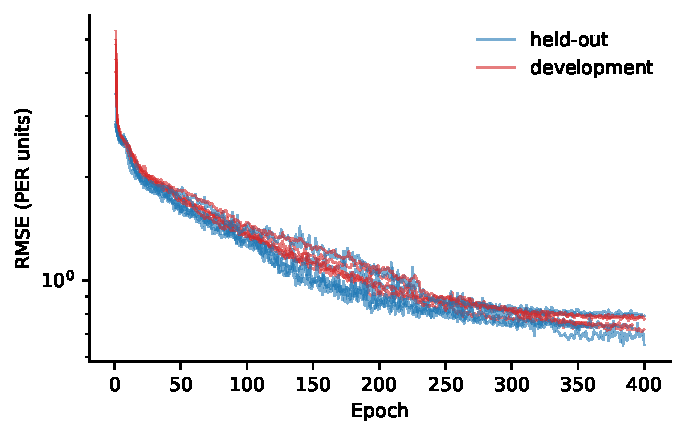
\includegraphics[width=0.55\textwidth]{figA1_training}
\caption{Development-set (red) and held-out (blue) reconstruction RMSE per epoch for five training seeds, $d=64$.}\label{fig:training}\end{figure}

\section{Single-run UMAP+HDBSCAN: selection and stability}\label{app:single}
\begin{table}[h]\centering\scriptsize
\caption{Configurations selected on the development set by three rules and their behaviour on held-out and refitted data. $^a$UMAP dimension / neighbours / minimum distance / HDBSCAN minimum cluster size / minimum samples. Sil.\ = Silhouette in the UMAP space, noise excluded.}
\label{tab:selection}
\resizebox{\textwidth}{!}{\begin{tabular}{llccccccccc}\toprule
 & & \multicolumn{4}{c}{Development (80\%)} & \multicolumn{3}{c}{Held-out (20\%)} & \multicolumn{2}{c}{Refit on all} \\ \cmidrule(lr){3-6}\cmidrule(lr){7-9}\cmidrule(lr){10-11}
Selection rule & Configuration$^a$ & $k$ & Noise \% & Sil. & DBCV & $k$ & Noise \% & Sil. & $k$ & Noise \% \\ \midrule
DBCV (prespecified) & 10/10/0.0/15/15 & 7 & 1 & 0.36 & 0.48 & 7 & 1 & 0.36 & 13 & 12 \\
Silhouette & 2/30/0.0/20/5 & 24 & 25 & 0.52 & 0.19 & 23 & 56 & 0.47 & 14 & 10 \\
Composite score (2025 version) & 2/15/0.0/40/5 & 14 & 13 & 0.43 & 0.17 & 14 & 29 & 0.42 & 7 & 3 \\
\bottomrule\end{tabular}}
\end{table}
\begin{table}[h]\centering\small
\caption{Reproducibility of single runs. ARI over UMAP seeds: mean (range) of pairwise ARI among ten UMAP random states, averaged over three autoencoder seeds. ARI over AE seeds: mean pairwise ARI among the three autoencoder seeds at a fixed UMAP seed. $^a$Configurations: \configList.}
\label{tab:stability}
\resizebox{\textwidth}{!}{\begin{tabular}{llccccc}\toprule
Config.$^a$ & Extraction & ARI, UMAP seeds (range) & ARI, AE seeds & $k$ range (median) & Noise \% & Largest cluster \% \\ \midrule
C1 & eom & 0.60 (0.03--0.95) & 0.38 & 2--19 (9) & 13 & 49 \\
C1 & leaf & 0.64 (0.50--0.75) & 0.23 & 15--20 (18) & 37 & 8 \\
C4 & eom & 0.66 (0.03--0.99) & 0.34 & 2--14 (8) & 5 & 63 \\
C4 & leaf & 0.32 (0.18--0.50) & 0.18 & 12--20 (16) & 28 & 9 \\
C2 & eom & 0.63 (0.03--0.95) & 0.31 & 3--18 (12) & 19 & 34 \\
C2 & leaf & 0.59 (0.44--0.71) & 0.25 & 14--19 (16) & 34 & 9 \\
C3 & eom & 0.44 (0.02--0.98) & 0.09 & 2--22 (18) & 20 & 33 \\
C3 & leaf & 0.57 (0.44--0.70) & 0.20 & 20--27 (23) & 35 & 6 \\
\bottomrule\end{tabular}}
\end{table}

\section{Consensus diagnostics, cross-representation agreement and macro-types}\label{app:k}
Table~\ref{tab:kcurve} lists PAC, consensus Silhouette and the share of stable players for every $k$. PAC decreases almost monotonically in $k$ for every representation, which is why it cannot select $k$ by itself and the consensus Silhouette was used; the PAC-minimum rule would select $k=12$ for every representation. Table~\ref{tab:crossrep} gives the agreement between representations at $k=8$, and Table~\ref{tab:profiles4} the rule-selected macro-types with their nesting of the fine types (Table~\ref{tab:nesting}).
\begin{table}[h]\centering\small
\caption{Consensus diagnostics by number of clusters $k$ for the summary-statistic representation and the five-seed autoencoder representation.}\label{tab:kcurve}
\begin{tabular}{ccccccc}\toprule
 & \multicolumn{3}{c}{Summary statistics} & \multicolumn{3}{c}{Autoencoder $d=64$, 5 seeds} \\ \cmidrule(lr){2-4}\cmidrule(lr){5-7}
$k$ & PAC & Sil.$_C$ & Stable \% & PAC & Sil.$_C$ & Stable \% \\ \midrule
2 & 0.04 & 0.98 & 100 & 0.41 & 0.80 & 97 \\
3 & 0.11 & 0.92 & 99 & 0.57 & 0.48 & 80 \\
4 & 0.08 & 0.93 & 99 & 0.57 & 0.39 & 69 \\
5 & 0.11 & 0.90 & 99 & 0.50 & 0.37 & 66 \\
6 & 0.17 & 0.83 & 98 & 0.42 & 0.38 & 65 \\
7 & 0.14 & 0.80 & 96 & 0.36 & 0.42 & 66 \\
8 & 0.07 & 0.90 & 99 & 0.32 & 0.44 & 67 \\
9 & 0.13 & 0.80 & 97 & 0.30 & 0.38 & 51 \\
10 & 0.17 & 0.61 & 88 & 0.27 & 0.36 & 49 \\
11 & 0.16 & 0.63 & 89 & 0.25 & 0.34 & 42 \\
12 & 0.15 & 0.59 & 87 & 0.23 & 0.34 & 42 \\
\bottomrule\end{tabular}
\end{table}
\begin{table}[h]\centering\small
\caption{Agreement (ARI) between the $k=8$ consensus partitions obtained from different representations of the same \nPlayers{} careers.}
\label{tab:crossrep}
\begin{tabular}{lccccccc}\toprule
 & Summary & Resampled & PCA & DTW & AE (5 seeds) & AE (seed 0) & AE+UMAP \\ \midrule
Summary & 1.00 &  &  &  &  &  &  \\
Resampled & 0.32 & 1.00 &  &  &  &  &  \\
PCA & 0.18 & 0.12 & 1.00 &  &  &  &  \\
DTW & 0.19 & 0.27 & 0.06 & 1.00 &  &  &  \\
AE (5 seeds) & 0.22 & 0.20 & 0.12 & 0.12 & 1.00 &  &  \\
AE (seed 0) & 0.20 & 0.18 & 0.12 & 0.13 & 0.57 & 1.00 &  \\
AE+UMAP & 0.19 & 0.15 & 0.11 & 0.04 & 0.29 & 0.20 & 1.00 \\
\bottomrule\end{tabular}
\end{table}
\label{app:nesting}
\begin{table}[h]\centering\scriptsize
\caption{Macro-types ($k=\mainK$, rule-selected) of the summary-statistic consensus. Stability = median player stability; PER, seasons and slope are cluster medians.}
\label{tab:profiles4}
\resizebox{\textwidth}{!}{\begin{tabular}{lcccccccclp{3.6cm}}\toprule
Type & $n$ & Stability & Mean PER & Peak PER & Seasons & Slope & All-Star \% & Career WS & Label (rule) & Nearest to medoid \\ \midrule
T1 & 369 & 0.98 & 16.5 & 20.4 & 12 & -0.30 & 52 & 52.5 & moderate-PER, long career, declining & Josh Smith, Amir Johnson, Eric Bledsoe \\
T2 & 560 & 0.98 & 12.5 & 16.2 & 11 & -0.34 & 8 & 24.7 & moderate-PER, long career, declining & Mike Sanders, Nick Young, Aaron Brooks \\
T3 & 444 & 0.96 & 10.6 & 13.0 & 3 & -0.86 & 1 & 3.0 & low-PER, short career, declining & Jonny Flynn, Anthony Jones, Litterial Green \\
T4 & 303 & 0.98 & 10.6 & 12.4 & 3 & +0.70 & 0 & 1.5 & low-PER, short career, rising & Qyntel Woods, Delaney Rudd, Larry Spriggs \\
\bottomrule\end{tabular}}
\end{table}
\begin{table}[h]\centering\small
\caption{Cross-tabulation of the eight fine types (rows) against the four macro-types (columns); \nestingPurity\% of players lie in the modal macro-type of their fine type (ARI between the two partitions \ariFourEight).}\label{tab:nesting}
\begin{tabular}{lrrrr}
\toprule
Macro-type & 1 & 2 & 3 & 4 \\
Fine type &  &  &  &  \\
\midrule
1 & 138 & 0 & 0 & 0 \\
2 & 101 & 30 & 35 & 0 \\
3 & 92 & 190 & 1 & 0 \\
4 & 38 & 45 & 5 & 53 \\
5 & 0 & 12 & 224 & 40 \\
6 & 0 & 283 & 50 & 6 \\
7 & 0 & 0 & 2 & 204 \\
8 & 0 & 0 & 127 & 0 \\
\bottomrule
\end{tabular}

\end{table}

\section{Internal indices in each method's own space}\label{app:internal}
Table~\ref{tab:internal} reports Silhouette, Calinski--Harabasz and Davies--Bouldin indices of each $k=8$ consensus partition in the space that the respective method clustered; they are not comparable across representations.
\begin{table}[h]\centering\small
\caption{Internal indices of the $k=8$ consensus partitions, computed in each representation's own (standardised) space.}\label{tab:internal}
\begin{tabular}{lccc}\toprule
Representation & Silhouette & Calinski--Harabasz & Davies--Bouldin \\ \midrule
Summary statistics, $k$-means & 0.19 & 395 & 1.40 \\
Resampled trajectory, $k$-means & 0.17 & 548 & 1.53 \\
PCA of resampled trajectory, $k$-means & 0.02 & 145 & 2.63 \\
Autoencoder $d=64$, 5 seeds (latent space) & 0.09 & 127 & 2.24 \\
\bottomrule\end{tabular}
\end{table}

\end{document}
